\documentclass[a4j,20pt,slide]{ltjsarticle}
\usepackage{url}%URL
\usepackage[pdfencoding=auto]{hyperref}%ハイパーリンク
\usepackage[dvips]{graphicx}%画像
\graphicspath{{./fig/}}%画像フォルダーの指定
\usepackage{here}%float環境の出力位置をコントロール
\usepackage{ascmac}
\usepackage{amssymb}
\usepackage{color}
\usepackage{booktabs}%罫線
\usepackage{menukeys}
\renewmenumacro{\directory}{pathswithfolder}
\usepackage{xcolor}
\hypersetup{
    colorlinks=true,
%    citebordercolor=green,
%    linkbordercolor=blue,
%    urlbordercolor=cyan,
}
\usepackage{listings}%ソースコード
\lstset{
  basicstyle={\normalsize\ttfamily},
  commentstyle=\color{blue},
  rulecolor=\color{black},
  frame={tb},
  backgroundcolor={\color[gray]{.97}},
  breaklines=true,
  columns=[l]{fullflexible},
  numberstyle={\scriptsize},
  keepspaces=true,
  showstringspaces=false
}
%キャプション表示設定
\usepackage{caption}
%\usepackage[labelformat=empty,labelsep=none]{caption}
\renewcommand{\figurename}{Fig.}
\renewcommand{\tablename}{Table.}
\renewcommand{\lstlistingname}{Code.}
%箇条書きの記号変更
\renewcommand{\labelitemii}{$\circ$}
\renewcommand{\labelitemiii}{$\triangleright$}
\renewcommand{\labelitemiv}{$\Rightarrow$}
%
\usepackage{geometry}
\geometry{textwidth=270mm, textheight=195mm}
%\renewcommand{\figurename}{Fig.}
%表紙用データ
\title{実践的構造解析ツールPrePoMaxを改めて使ってみた!}
\author{龍野 潤/Jun Tatsuno\\(CAE懇話会・オープンCAE学会)}
\date{2021年10月3日\\第22回オープンCAE勉強会@関東(構造など)}
\pagestyle{plain}
%
\begin{document}
\maketitle
%
\tableofcontents
%
\section{CalculiXとは}
\begin{itemize}
	\item フリーソフトウェアによる3次元構造用有限要素プログラム
	      \begin{itemize}
		      \item CCX(\textbf{C}alculiX \textbf{C}runchi\textbf{X}):有限要素ソルバー
		      \item CGX(\textbf{C}alculiX \textbf{G}raphi\textbf{X}):プリ・ポストプロセッサ
	      \end{itemize}
	\item OS:Linux / Windows\footnote{Convergent Mechanical社はWindowsオペレーティングシステムに移植}
	\item ライセンス:GPLライセンス
	\item 現在の最新版は2.17(2020年7月26日公開)
	\item Abaqus と同様の入力形式を使用
\end{itemize}
\vspace{-\baselineskip}
\begin{figure}[H]
	\begin{minipage}{0.49\hsize}
		\caption{CalculiX Command Window}
		%			\label{}
		\centering
		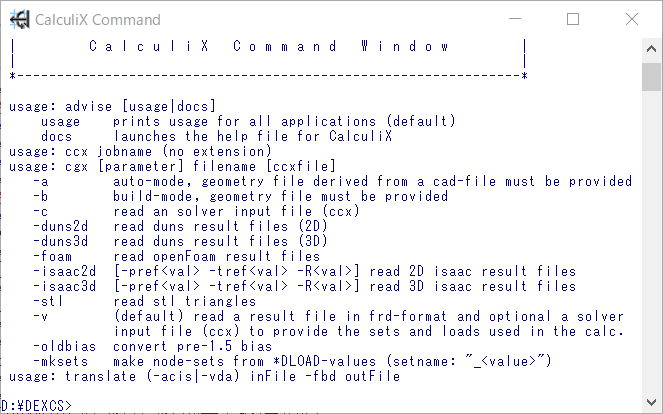
\includegraphics[width=.9\columnwidth]{fig/CCX.png}
	\end{minipage}
	\begin{minipage}{0.49\hsize}
		\caption{CGX}
		%		 	\label{}
		\centering
		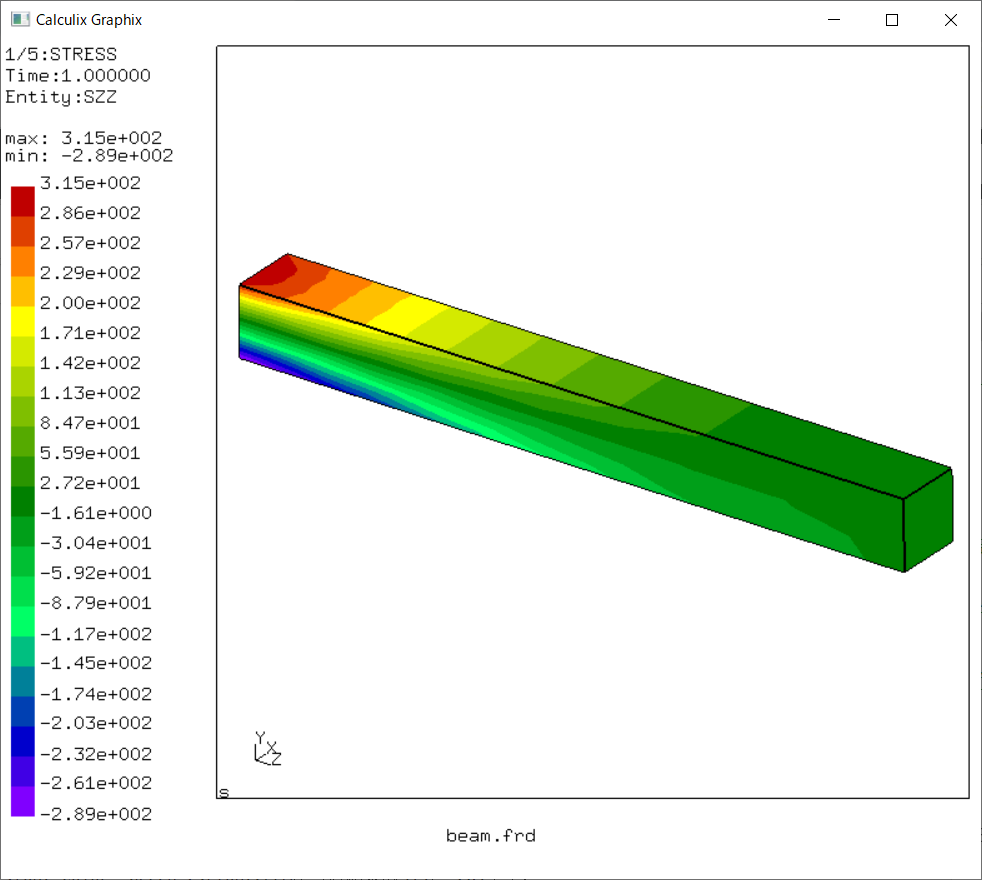
\includegraphics[width=.65\columnwidth]{fig/CGX.png}
	\end{minipage}
\end{figure}
%
\section{CalculiXのデータ設定例}
\href{http://www.bconverged.com/content/calculix/doc/GettingStarted.pdf}{Getting Started Guide}での設定例
\begin{lstlisting}[caption=beam.inp]
*INCLUDE, INPUT=all.msh
*INCLUDE, INPUT=fix1.nam
*INCLUDE, INPUT=fix2.nam
*INCLUDE, INPUT=fix3.nam
*MATERIAL, Name=steel
*ELASTIC	# 等方性弾性材料
  28000000, 0.3	# ヤング率、ポアソン比
*SOLID SECTION, Elset=Eall, Material=steel	# 材料の割り当て
*STEP
*STATIC	# 静的線形構造解析
*BOUNDARY	# 変位拘束条件
  Nfix1,3,3,0
  Nfix2,2,3,0
  Nfix3,1,3,0
*DLOAD	# 分布荷重条件
*INCLUDE, INPUT=load.dlo
*NODE FILE
  U
*EL FILE
  S, E
*END STEP
\end{lstlisting}
%
\section{PrePoMaxとは}\label{sec:1.0}
PrePoMaxは、FEMワークフローを高速化するための最新のユーザーインタフェースに基づくCalculix FEMソルバー用のオープンソースのプリプロセッサおよびポストプロセッサです。
\begin{itemize}
	\item CADジオメトリサポート
	      \begin{itemize}
		      \item PrePoMaxでは、交換可能なさまざまなCADフォーマットや、3Dプリントに使用されるステレオリソグラフィーの.stlファイルからジオメトリをインポートできます。
		      \item このCADサポートは、オープンソースのOpen Cascadeプラットフォームをベースにしています。
	      \end{itemize}
	\item ソリッドとシェルのジオメトリのメッシュ分割
	      \begin{itemize}
		      \item PrePoMaxでは、線形および二次の有限要素を使用して、ソリッドまたはシェルベースのジオメトリをメッシュ分割できます。
		      \item ファイルからの有限要素メッシュのインポートにも対応しています。
		      \item メッシュ分割にはオープンソースのNetgenライブラリを使用しています。
	      \end{itemize}
	\item ジオメトリとメッシュベースのフィーチャ定義
	      \begin{itemize}
		      \item PrePoMaxでは、ジオメトリや有限要素メッシュの選択に基づいて、さまざまなFEM機能に必要な節点セット、要素セット、サーフェスを作成できます。
	      \end{itemize}
	\item 結果の可視化
	      \begin{itemize}
		      \item PrePoMaxでは、3Dスカラーフィールドを使用して、または履歴出力を表現するための2Dプロッティングツールを使用して、結果を可視化できます。
	      \end{itemize}
\end{itemize}
%
\section{機能}\label{sec:2.0}
PrePoMaxには、さまざまなFEMモデルの準備、求解、ポストプロセスに必要な多くの機能が搭載されています。もっとも重要な機能の概要は以下の通りです。
\begin{itemize}
	\item 解析の種類
	      \begin{itemize}
		      \item 静的線形解析
		      \item 幾何学的非線形、材料非線形、接触非線形を含む静的非線形解析
		      \item 周波数解析
		      \item 座屈解析
		      \item 熱伝達解析
		      \item 非連成温度-変位解析
		      \item 連成温度-変位解析
	      \end{itemize}
	\item ジオメトリベースのメッシュ生成
	      \begin{itemize}
		      \item シェルCADパーツ - 三角形と四角形のシェル要素
		      \item シェル.stlパーツ - 三角形と四角形のシェル要素
		      \item ソリッドCADパーツ - 四面体ソリッド要素
		      \item ソリッド.stlパーツ - 四面体ソリッド要素
		      \item 頂点、エッジ、サーフェスに基づいて定義されたすべてのメッシュタイプで、メッシュの再分割が可能です。
	      \end{itemize}
	\item 有限要素の種類
	      \begin{itemize}
		      \item 線形と二次の三角形シェル要素(Calculixの実装)
		      \item 線形と二次の四角形シェル要素(Calculixの実装)
		      \item 線形と二次の四面体ソリッド要素
		      \item 線形と二次のウェッジソリッド要素(メッシュインポートのみ)
		      \item 線形と二次の六面体ソリッド要素(メッシュインポートのみ)
	      \end{itemize}
	\item アセンブリの接続
	      \begin{itemize}
		      \item 基準点を用いた剛体接続
		      \item タイ接続
		      \item 摩擦あり接触
	      \end{itemize}
	\item 材料モデル
	      \begin{itemize}
		      \item 編集可能な素材ライブラリを内蔵
		      \item 線形弾性材料モデル(温度依存性)
		      \item 等方または移動硬化則を伴う弾塑性材料モデル(温度依存性)
	      \end{itemize}
\end{itemize}
\section{PrePoMaxとCalculiXの構造と連携}
PrePoMaxとCalculiXの関係は、FemapとNastranの関係とまったく同じです。
PrePoMaxはプリ・ポストプロセッサーです。
つまり計算のためのモデルの準備と結果の表示を行います。
CalculiXはFEM解析のみを行います。
\begin{figure}[H]
	\centering
	\caption{PrePoMaxとCalculiXの関係}
	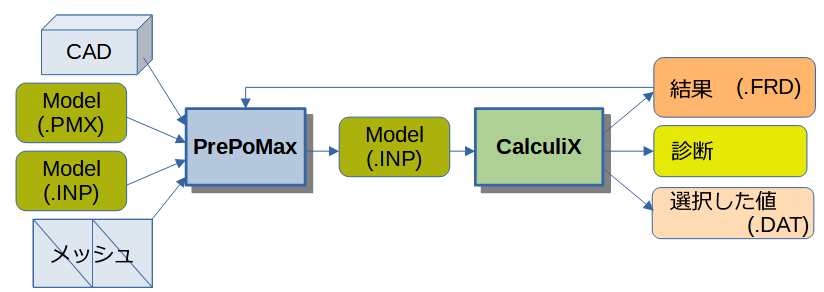
\includegraphics[width=.8\columnwidth]{fig/PrePoMax2CalculiX.png}
	\label{fig:019}
\end{figure}
\begin{itemize}
	\item PrePoMaxの入力ファイル
	      \begin{itemize}
		      \item FEMモデルファイル(CADモデル、FEMモデルを含む独自のPMX形式)
		      \item FEMモデルファイル(Abaqus/CalculiXプログラム形式)
		      \item CADファイル(BRep、IGES、STEP、STL形式)
		      \item 有限要素メッシュファイル(NEU、VOL、Mmg形式)
		      \item CalculiXの計算結果ファイル
	      \end{itemize}
	\item PrePoMax出力ファイル
	      \begin{itemize}
		      \item CalculiX用ファイル(.inp)
	      \end{itemize}
	\item CalculiXの出力ファイル
	      \begin{itemize}
		      \item メッシュ全体の計算結果のファイル(.frd)
		      \item 選択された節点または要素のセットに対するオプションの結果を含むテキストファイル(.dat)
		      \item 診断ファイル(.cvg、.12d、.out \ldots)
	      \end{itemize}
\end{itemize}
%
\subsection{前提条件}
PrePoMaxは、Microsoft .NET Framework 4.5.1をベースにしており、PrePoMaxを動作させるためにはコンピュータにインストールする必要があります。
\subsection{ソースコード}
PrePoMaxはフリーソフトウェアです。Free Software Foundationが発行したGNU General Public License, version 3の条項に基づいて、再配布や変更を行うことができます。
PrePoMaxのソースコードはGitLabで公開されています: \href{https://gitlab.com/MatejB/PrePoMax}{https://gitlab.com/MatejB/PrePoMax}
%
\section{解析事例}
\subsection{圧力荷重を受ける分割リング}
\begin{itemize}
	\item モデル形状(外径150mm、内径90mm、厚さ20mm)
	\item 最大要素サイズ:3mm
	\item 材料定数
	      \begin{itemize}
		      \item ヤング率:210,000MPa
		      \item ポアソン比:0.3
	      \end{itemize}
	\item 拘束条件:固定(下側の面)
	\item 荷重条件:20MPa(上側の面)
\end{itemize}
\vspace{-\baselineskip}
\begin{figure}[H]
	%
	\begin{minipage}{.49\hsize}
		\caption{境界条件}
		\label{01-01}
		\centering
		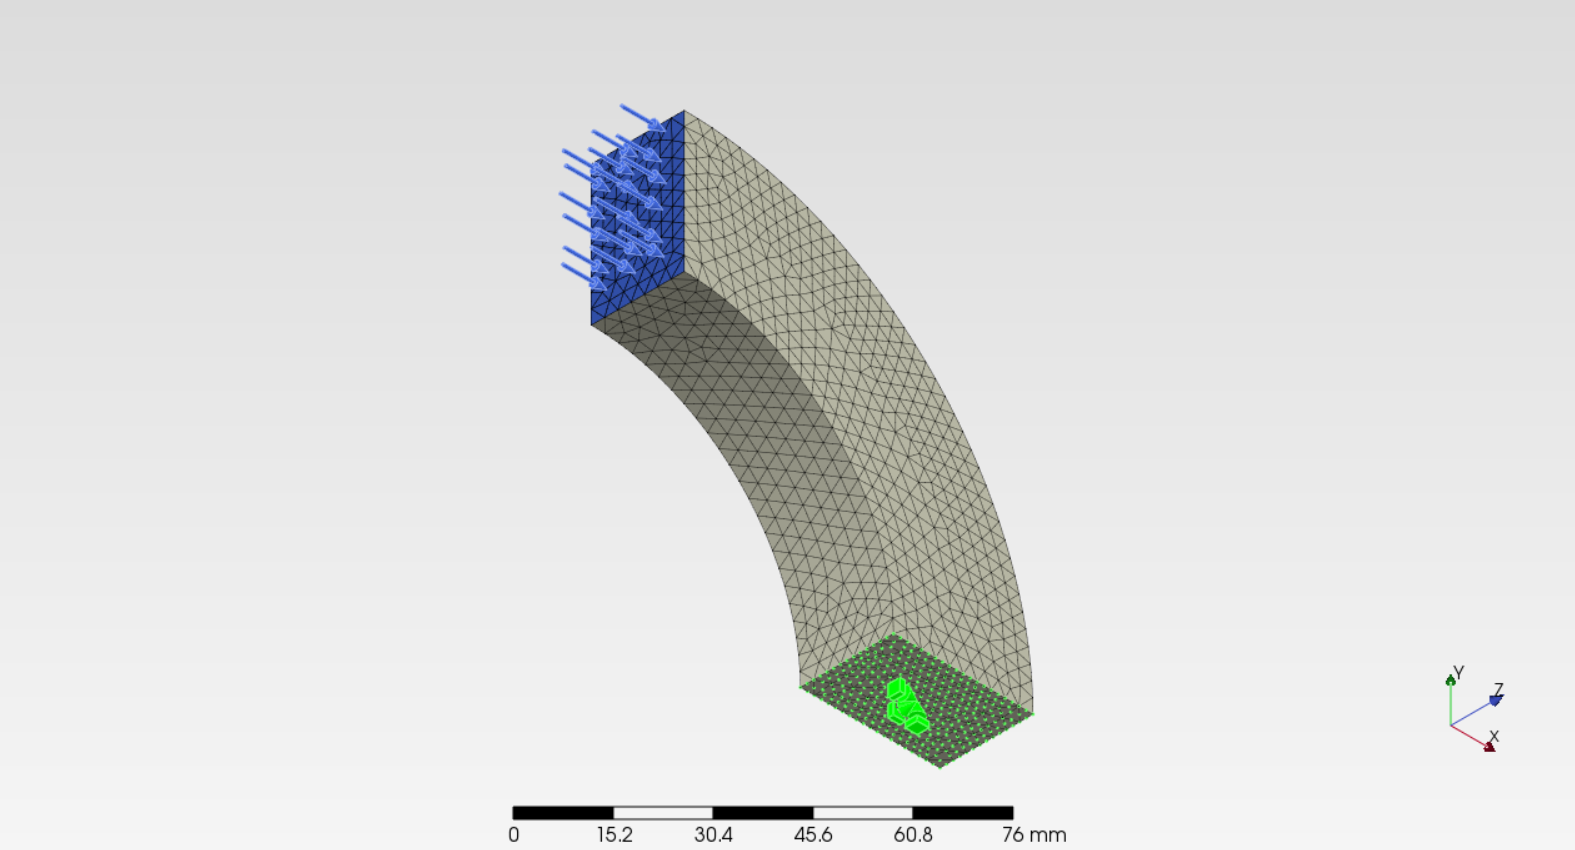
\includegraphics[width=.95\columnwidth]{fig/01-01.png}
	\end{minipage}
	%
	\begin{minipage}{.49\hsize}
		\caption{解析結果}
		\label{01-02}
		\centering
		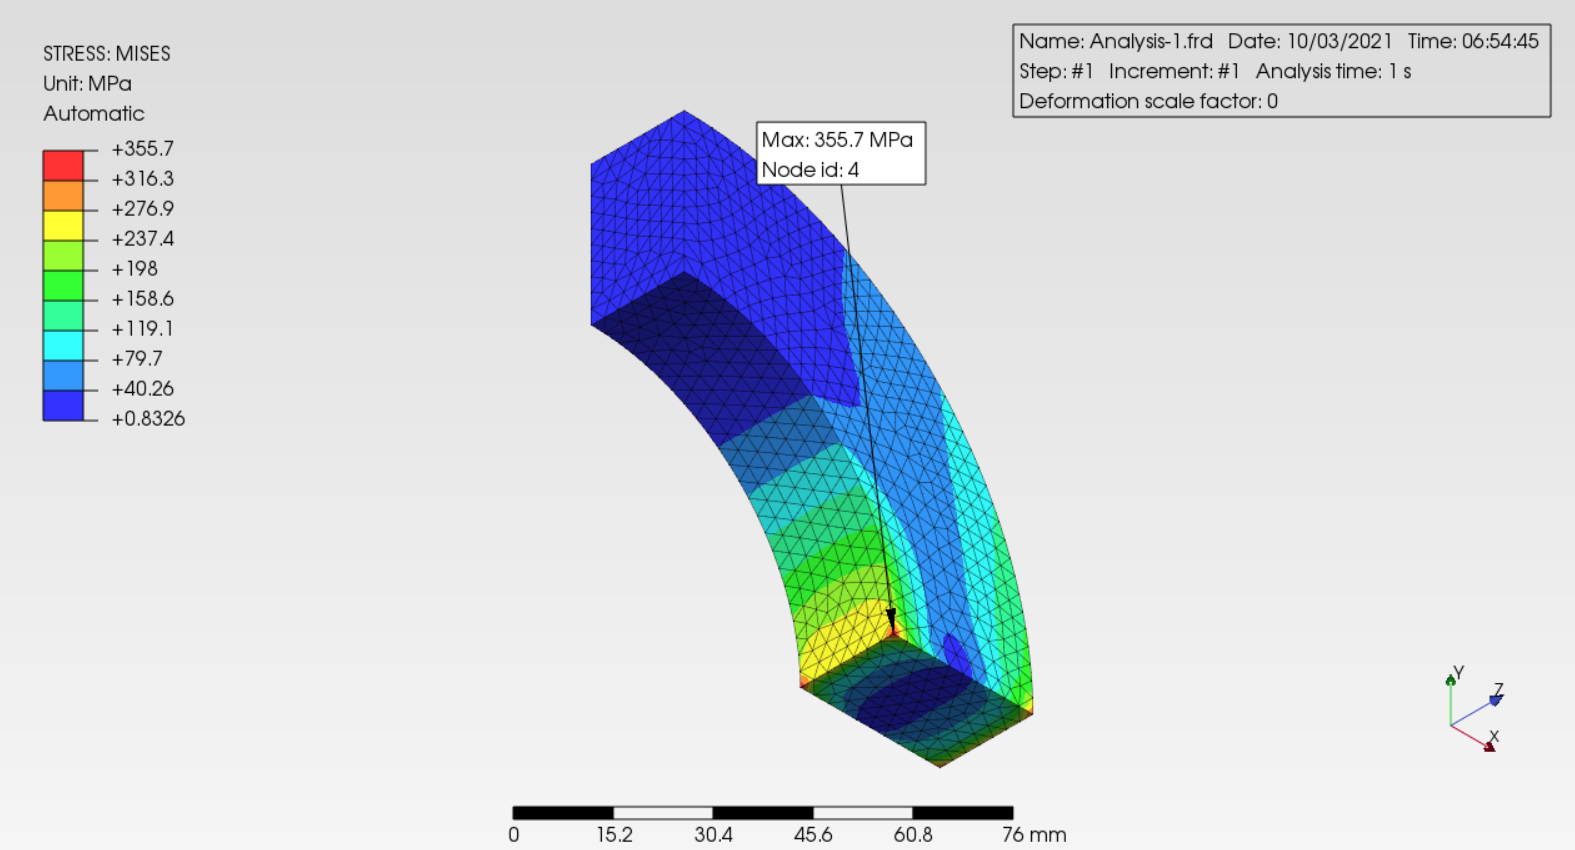
\includegraphics[width=.95\columnwidth]{fig/01-02.png}
	\end{minipage}
\end{figure}
\clearpage
%
\subsection{荷重を受けるシャフト}
\begin{itemize}
	\item モデル形状(直径50mm、長さ200mm)
	\item 最大要素サイズ:4mm
	\item 材料定数
	      \begin{itemize}
		      \item ヤング率:210,000MPa
		      \item ポアソン比:0.3
	      \end{itemize}
	\item 拘束条件:固定(シャフトの片側の端面)
	\item 荷重条件:シャフトの軸に垂直方向に-500N(固定拘束とは反対側の端面)
\end{itemize}
\vspace{-\baselineskip}
\begin{figure}[H]
	%
	\begin{minipage}{.49\hsize}
		\caption{境界条件}
		\label{02-01}
		\centering
		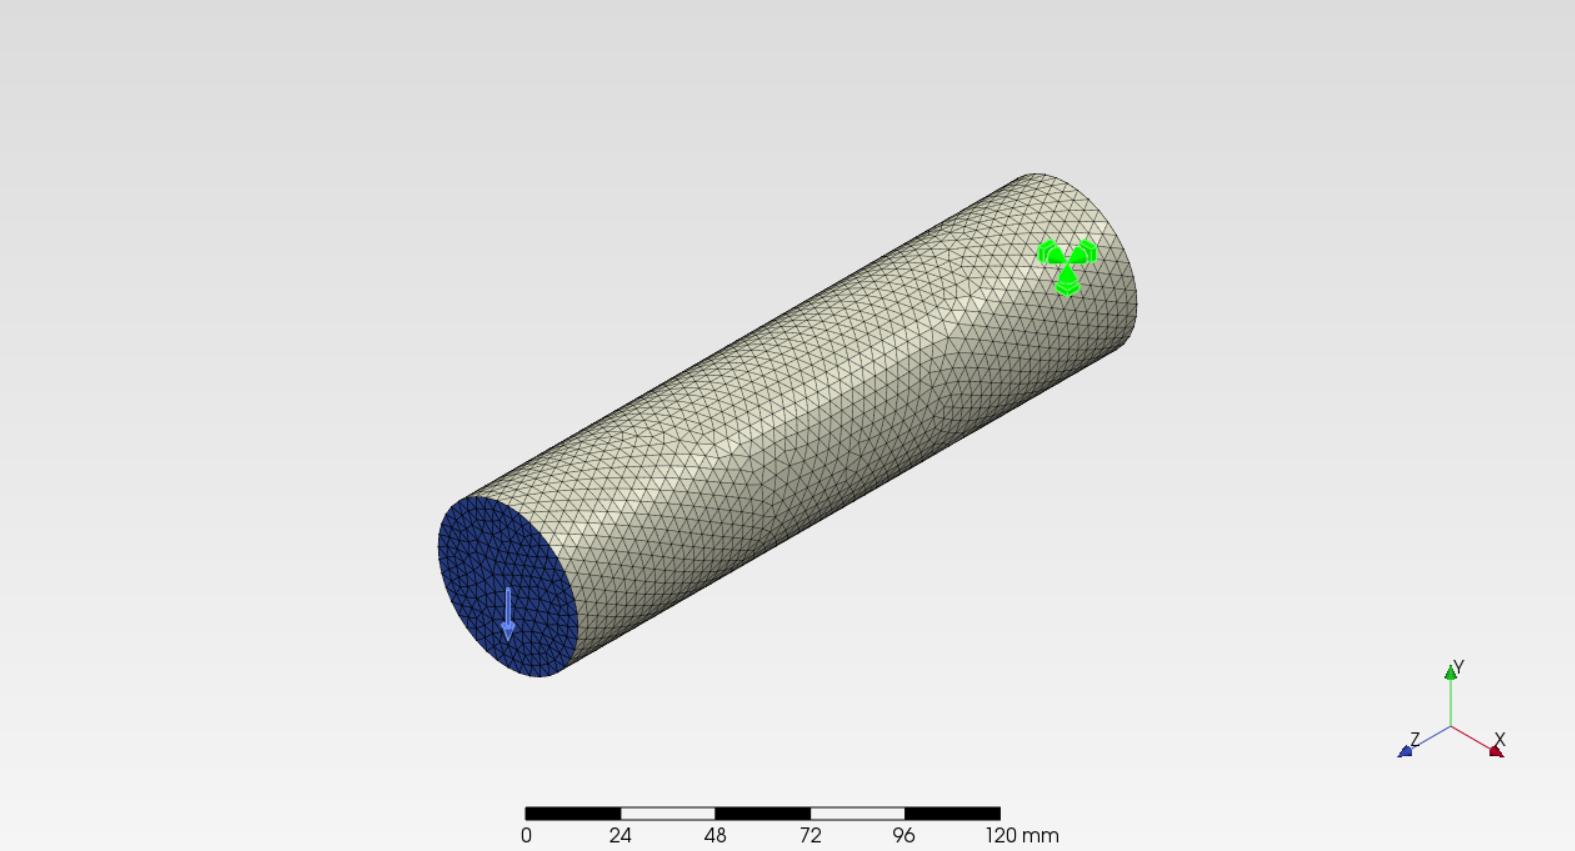
\includegraphics[width=.95\columnwidth]{fig/02-01.png}
	\end{minipage}
	%
	\begin{minipage}{.49\hsize}
		\caption{解析結果}
		\label{02-02}
		\centering
		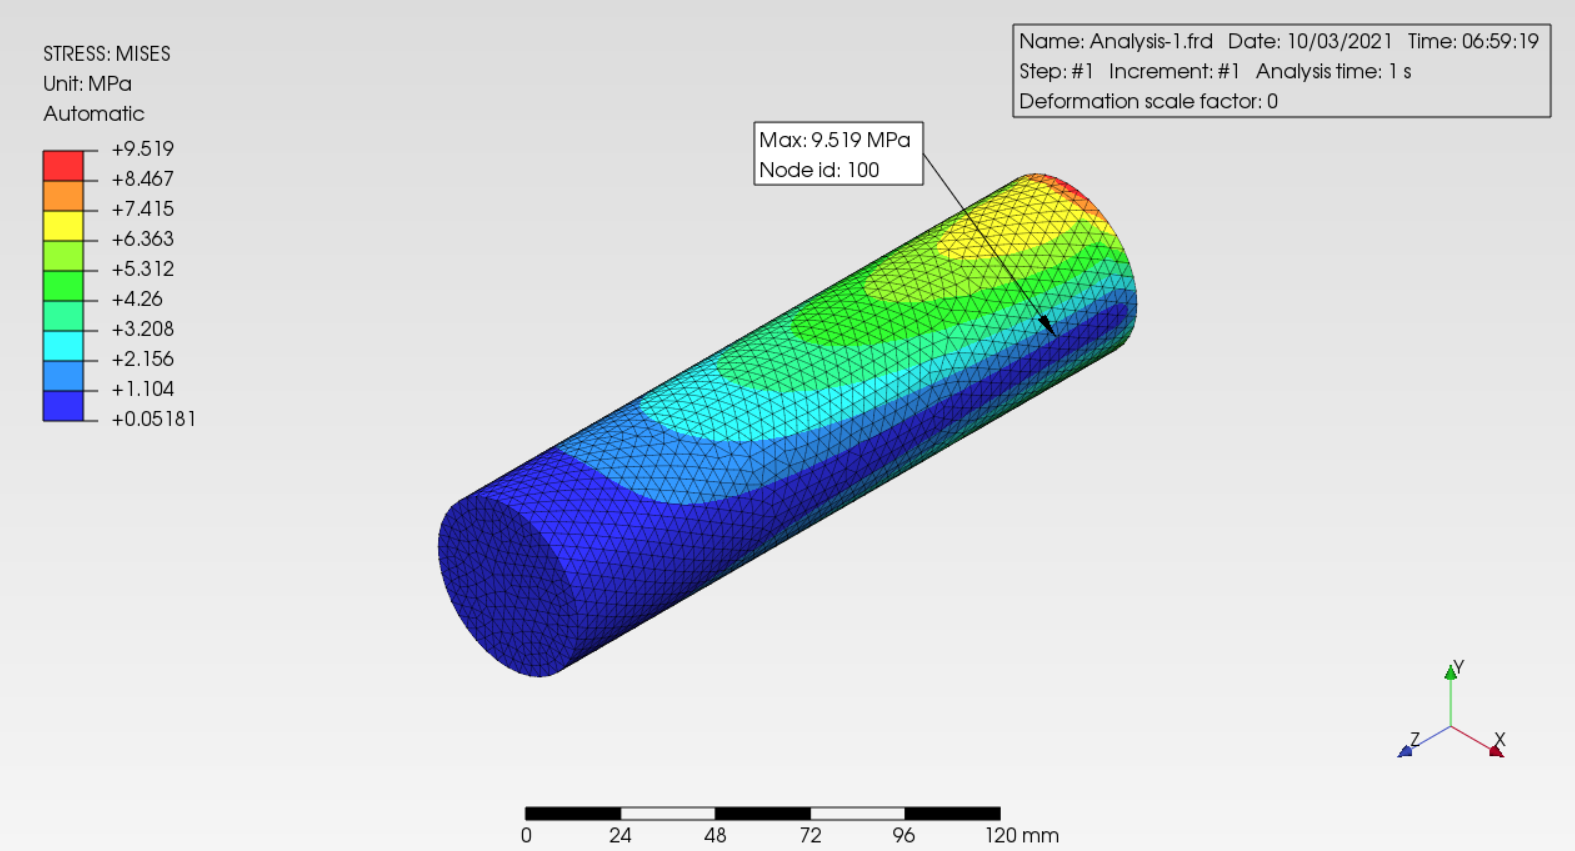
\includegraphics[width=.95\columnwidth]{fig/02-02.png}
	\end{minipage}
\end{figure}
\clearpage
%
\subsection{楕円形の棒のねじり}\label{sec:6.3}
\begin{itemize}
	\item モデル形状(長軸:200mm、短軸100 mm、長さ1,000mm)
	\item 最大要素サイズ:10mm
	\item 材料定数
	      \begin{itemize}
		      \item ヤング率:210,000MPa
		      \item ポアソン比:0.3
	      \end{itemize}
	\item 拘束条件:固定(楕円形の棒の片側の端面)
	\item 荷重条件:全荷重集中負荷1,000,000 Nmm(固定拘束とは反対側の端面の中心点)
\end{itemize}
\vspace{-\baselineskip}
\begin{figure}[H]
	%
	\begin{minipage}{.49\hsize}
		\caption{境界条件}
		\label{03-01}
		\centering
		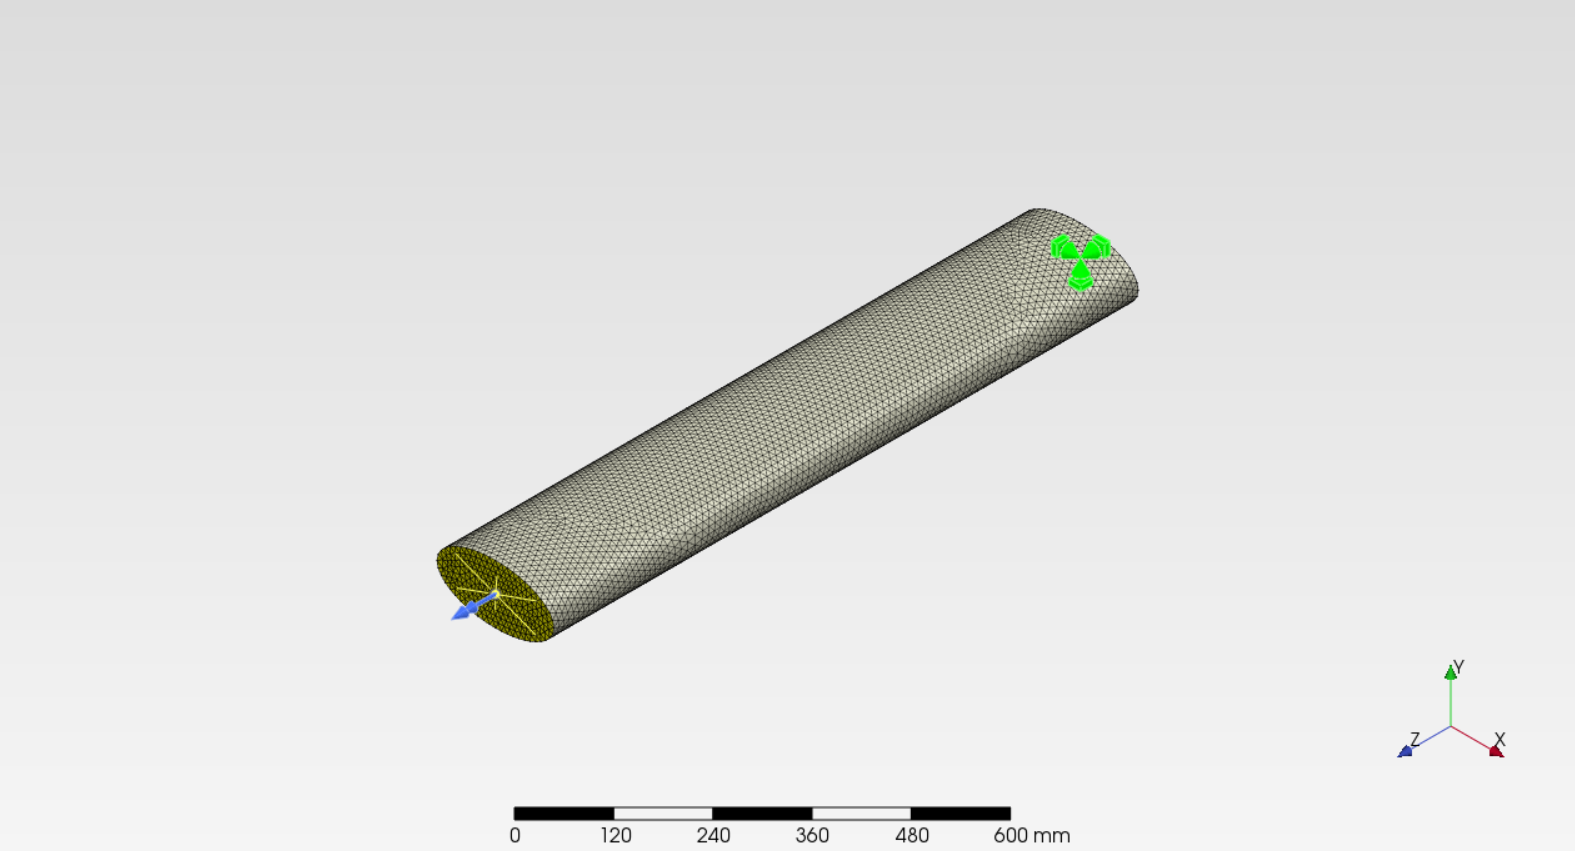
\includegraphics[width=.95\columnwidth]{fig/03-01.png}
	\end{minipage}
	%
	\begin{minipage}{.49\hsize}
		\caption{解析結果}
		\label{03-02}
		\centering
		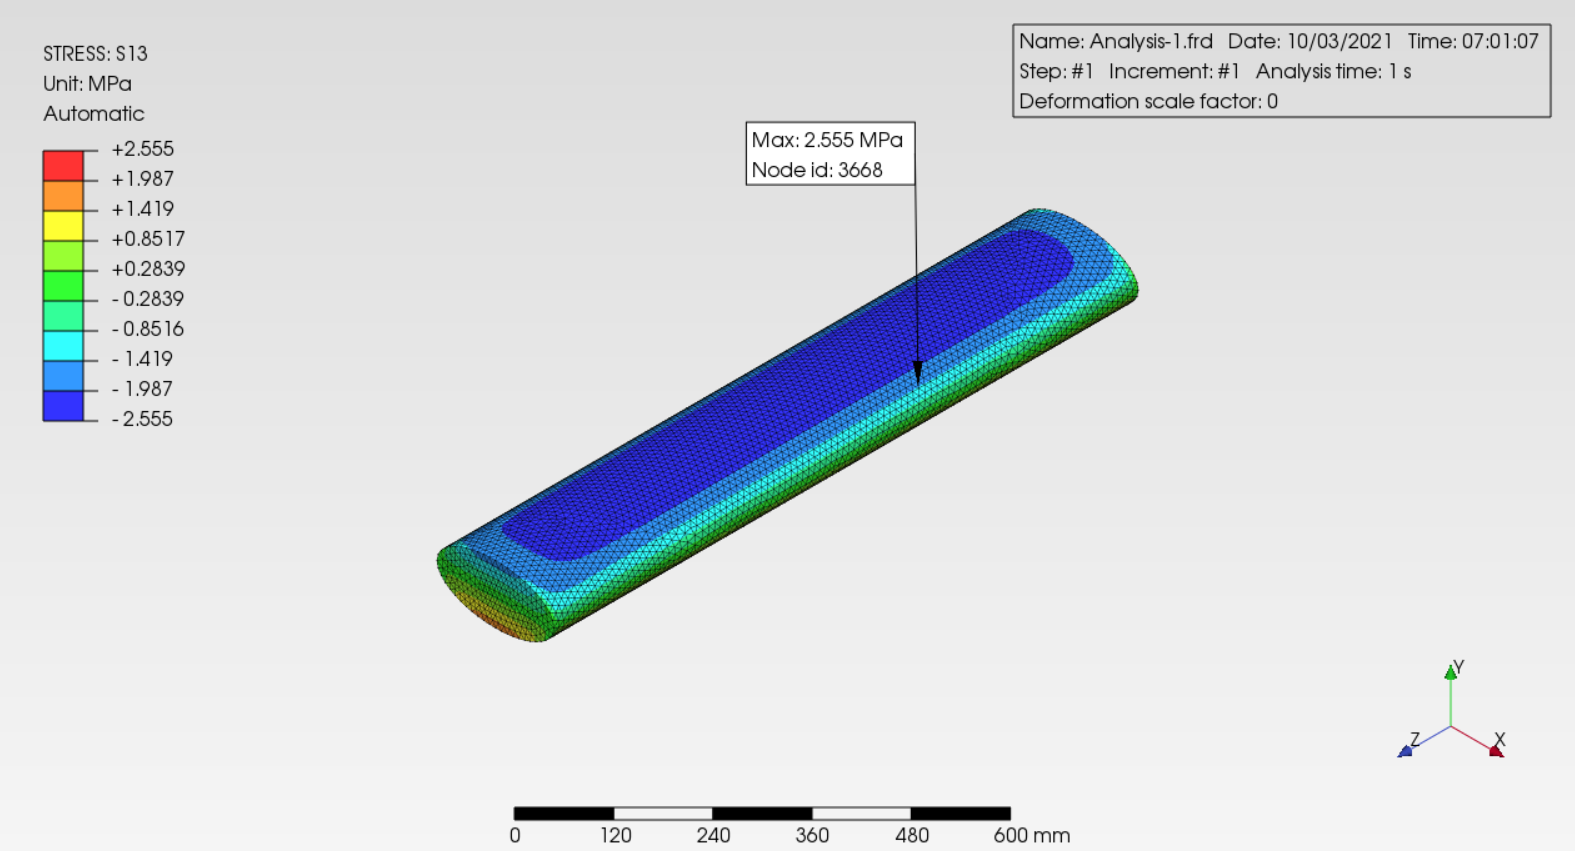
\includegraphics[width=.95\columnwidth]{fig/03-02.png}
	\end{minipage}
\end{figure}
\clearpage
%
\subsection{ねじりと曲げを受ける長方形の棒}
\begin{itemize}
	\item モデル形状(断面 200x300mmの長方形、長さ1,400 mm)
	\item 最大要素サイズ:30mm
	\item 材料定数
	      \begin{itemize}
		      \item ヤング率:180,000MPa
		      \item ポアソン比:0.25
	      \end{itemize}
	\item 拘束条件:固定(長方形の棒の片側の端面)
	\item 荷重条件:棒の軸に垂直な方向に-8,000N(座標(500,0,1400)の基準点から固定拘束とは反対側の端面へ)
\end{itemize}
\vspace{-\baselineskip}
\begin{figure}[H]
	%
	\begin{minipage}{.49\hsize}
		\caption{境界条件}
		\label{04-01}
		\centering
		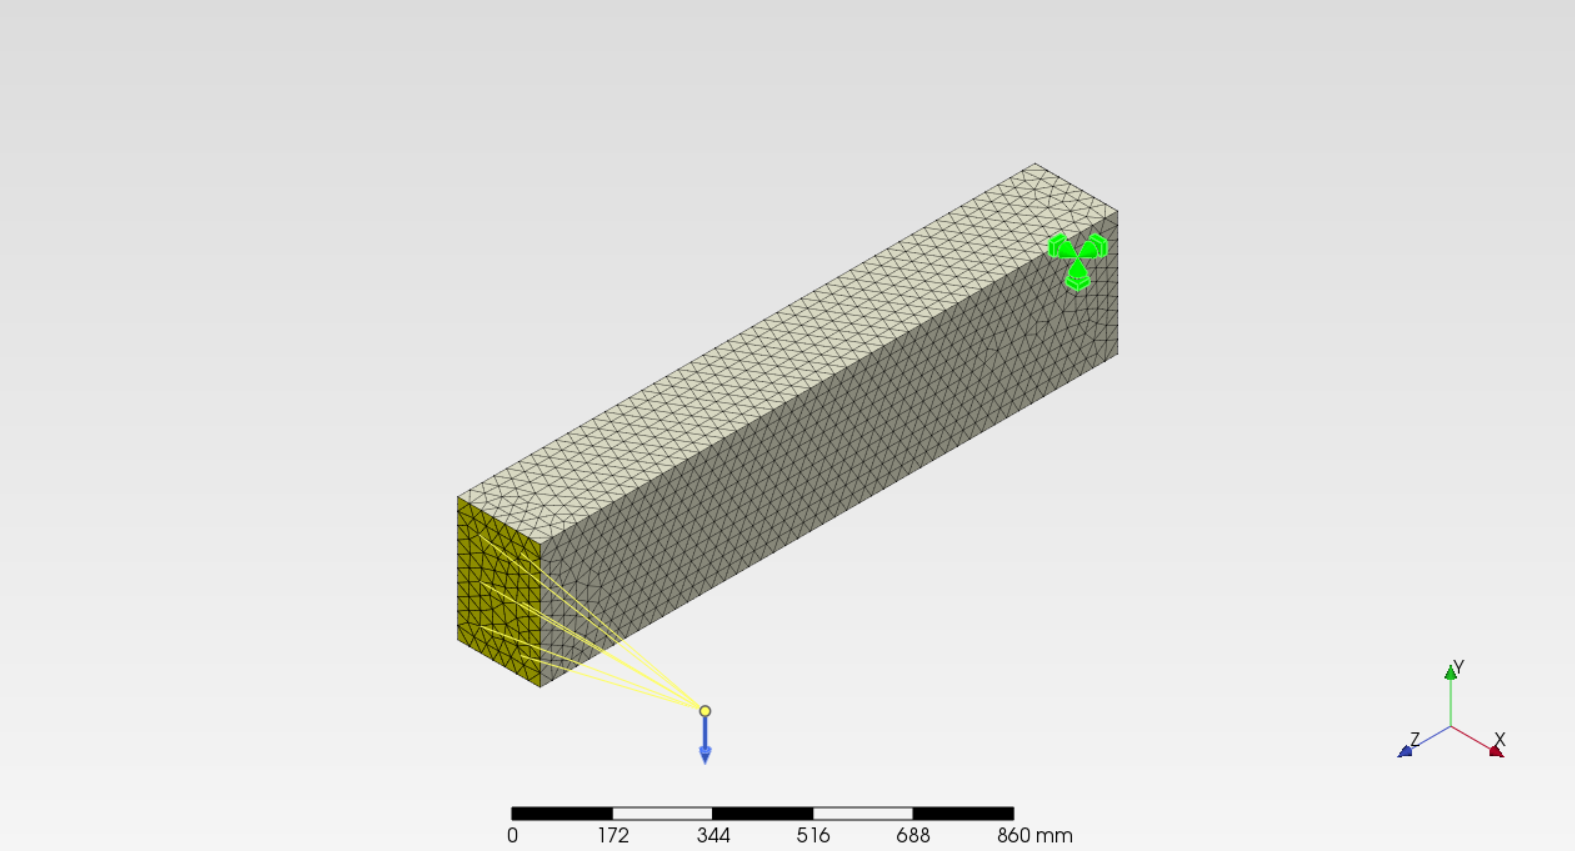
\includegraphics[width=.95\columnwidth]{fig/04-01.png}
	\end{minipage}
	%
	\begin{minipage}{.49\hsize}
		\caption{解析結果}
		\label{04-02}
		\centering
		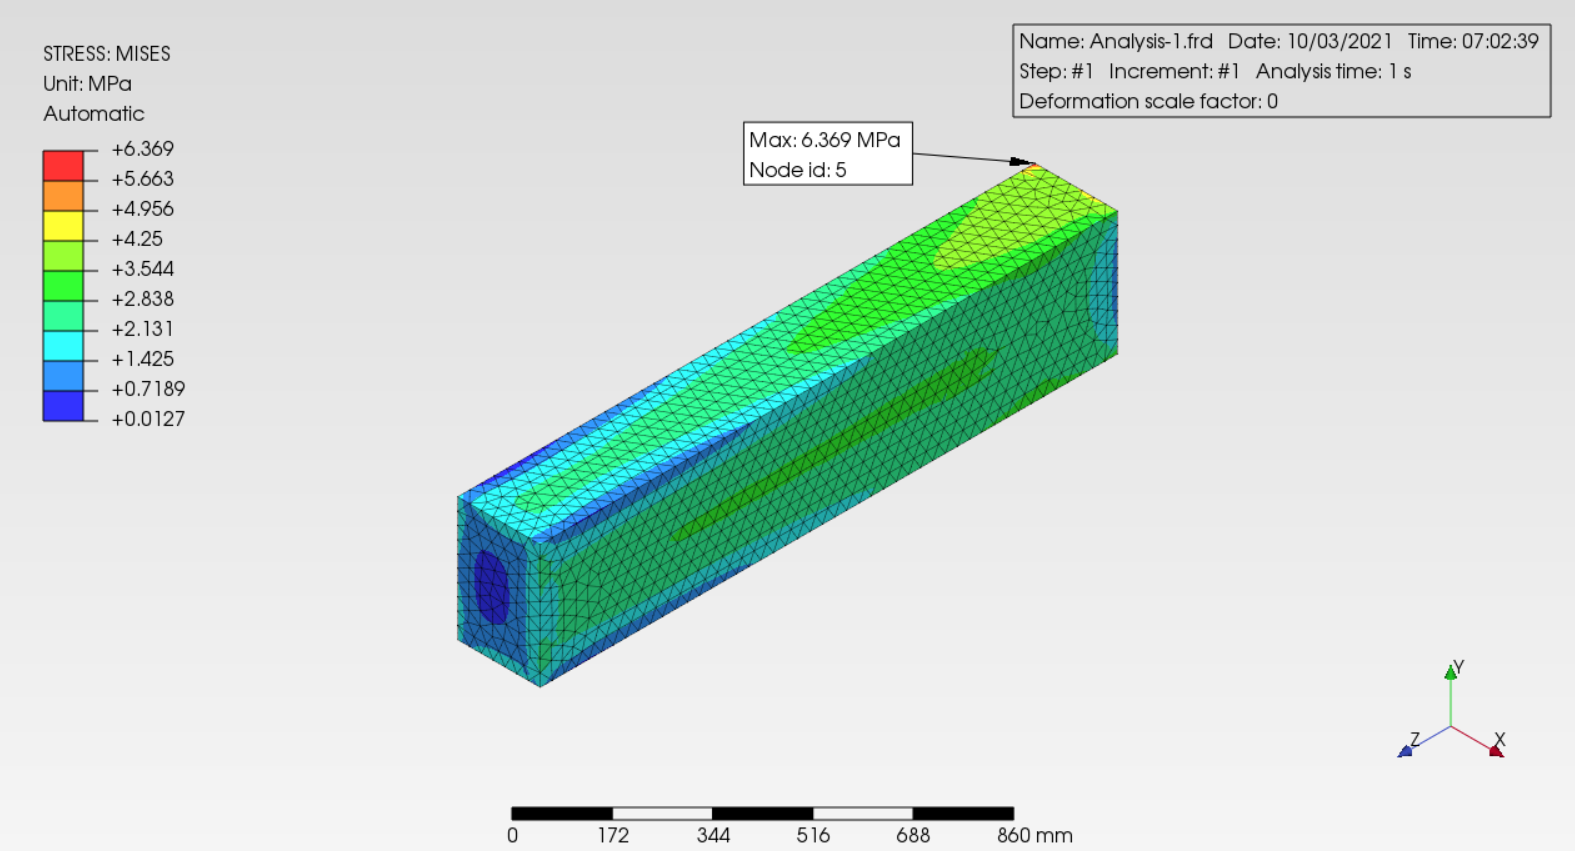
\includegraphics[width=.95\columnwidth]{fig/04-02.png}
	\end{minipage}
\end{figure}
\clearpage
%
\subsection{2つの円柱のアセンブリ}
\begin{itemize}
	\item モデル形状(太い円柱:直径80mm×長さ100mm、細い円柱:直径50mm×長さ120mm)
	\item 最大要素サイズ:5mm
	\item 材料定数
	      \begin{itemize}
		      \item ヤング率:180,000MPa
		      \item ポアソン比:0.25
	      \end{itemize}
	\item 拘束条件:固定(太い円柱の端面)
	\item 荷重条件:30MPa(細い円柱の端面)
	\item 接触条件:結合(2つの円柱が互いに接する面)
\end{itemize}
\vspace{-\baselineskip}
\begin{figure}[H]
	%
	\begin{minipage}{.49\hsize}
		\caption{境界条件}
		\label{05-01}
		\centering
		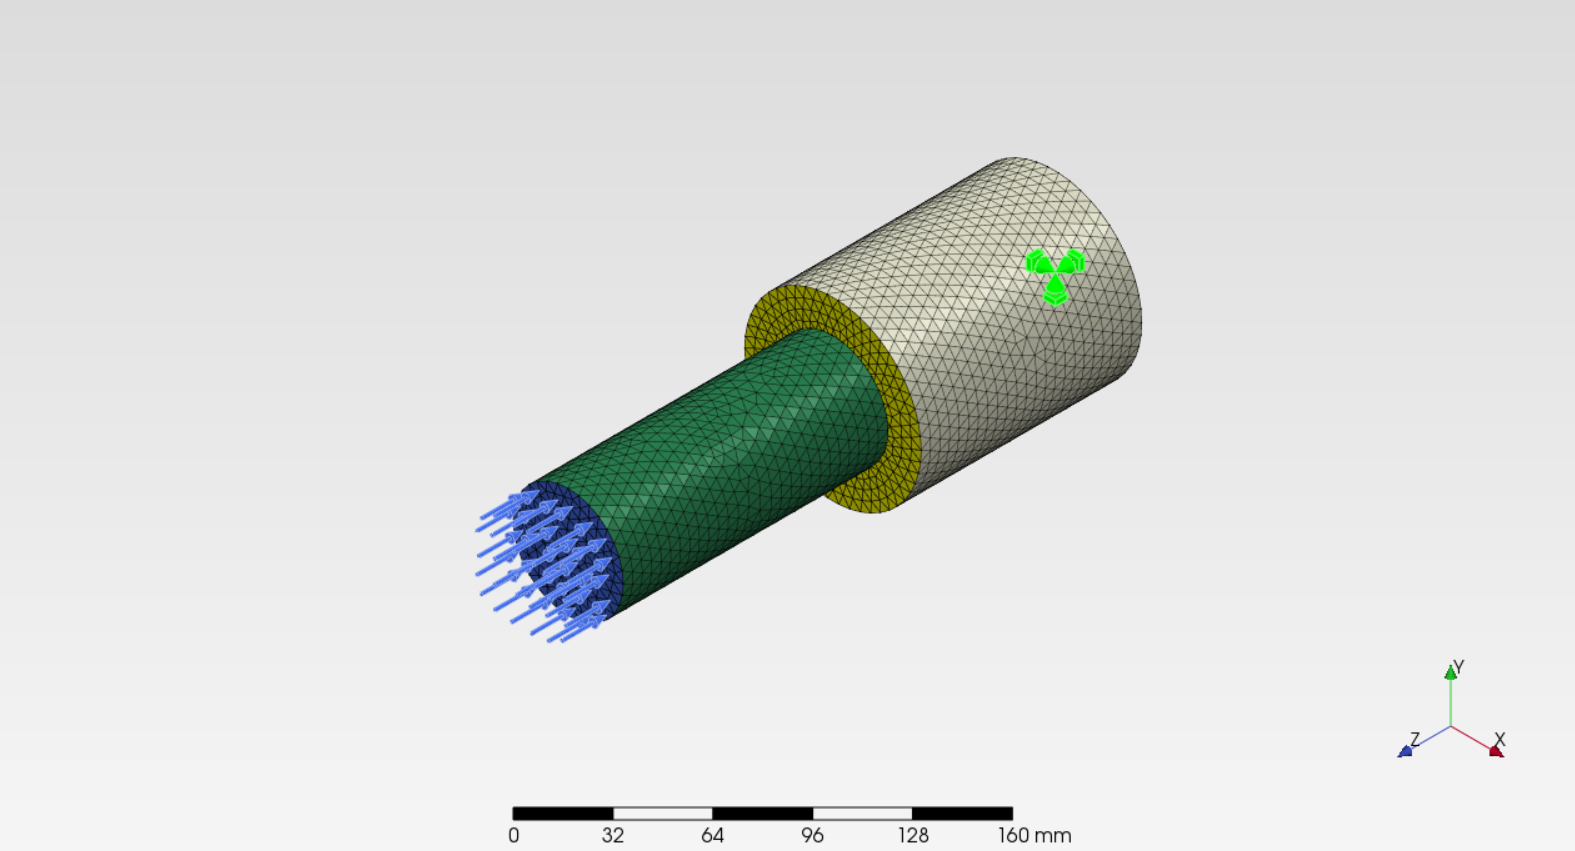
\includegraphics[width=.95\columnwidth]{fig/05-01.png}
	\end{minipage}
	%
	\begin{minipage}{.49\hsize}
		\caption{解析結果}
		\label{05-02}
		\centering
		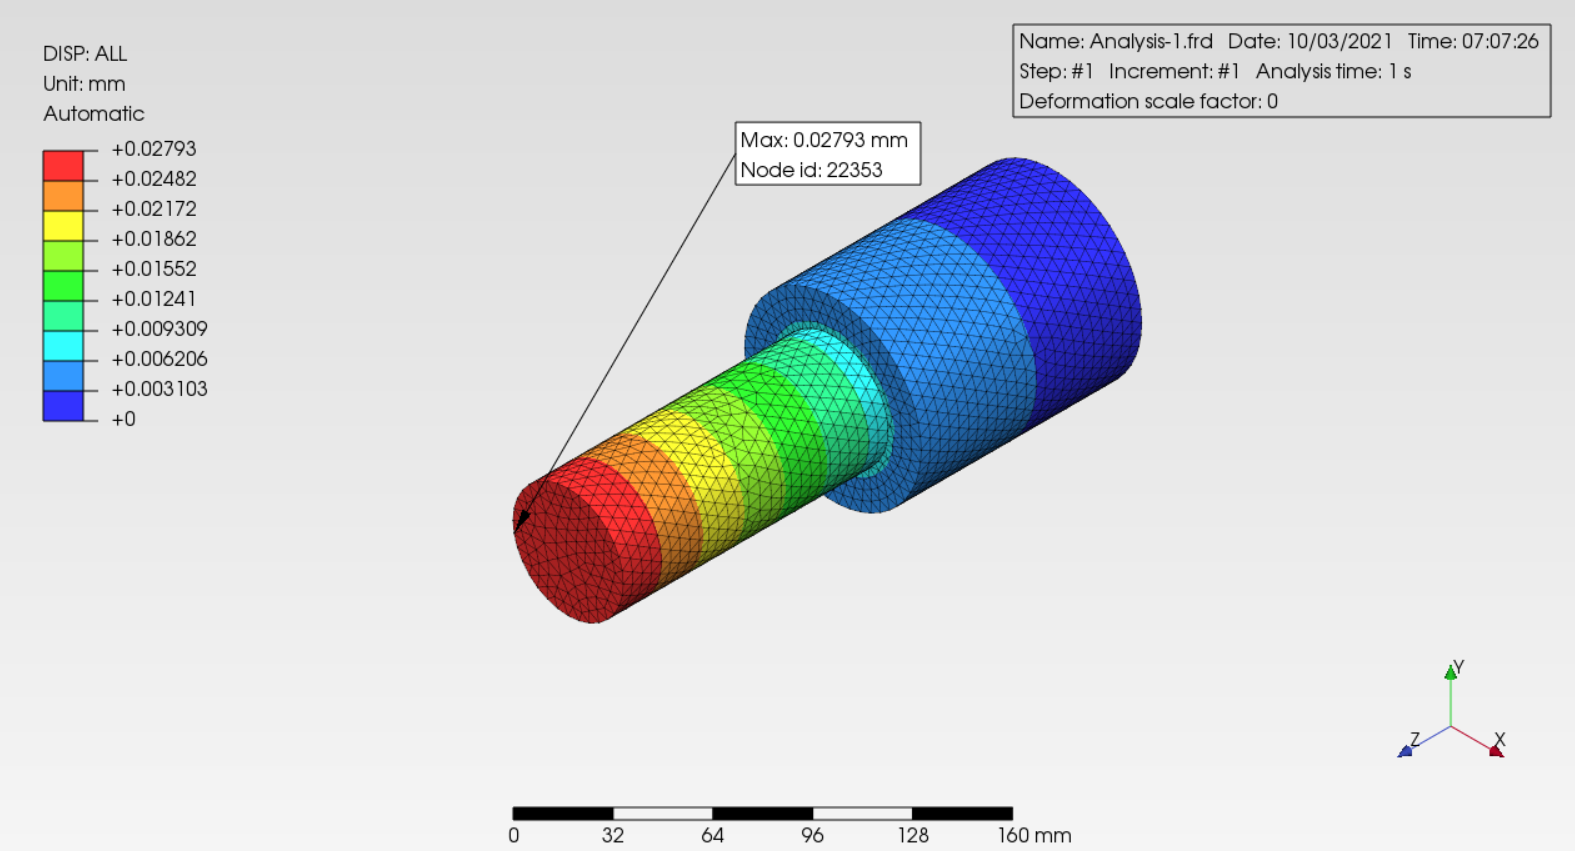
\includegraphics[width=.95\columnwidth]{fig/05-02.png}
	\end{minipage}
\end{figure}
%
\subsection{梁のモーダル解析}
\begin{itemize}
	\item モデル形状(断面:正方形40mm、長さ:1000mm)
	\item 最大要素サイズ:10mm
	\item 材料定数
	      \begin{itemize}
		      \item ヤング率:210,000MPa
		      \item ポアソン比:0.3
		      \item 密度:7.85e-9tont/mm3
	      \end{itemize}
	\item 拘束条件:一方の端の断面の下部エッジ(U1、U2、U3を固定)、反対側の断面の下部エッジ(U1、U2を固定)
\end{itemize}
\vspace{-\baselineskip}
\begin{figure}[H]
	%
	\begin{minipage}{.49\hsize}
		\caption{境界条件}
		\label{06-01}
		\centering
		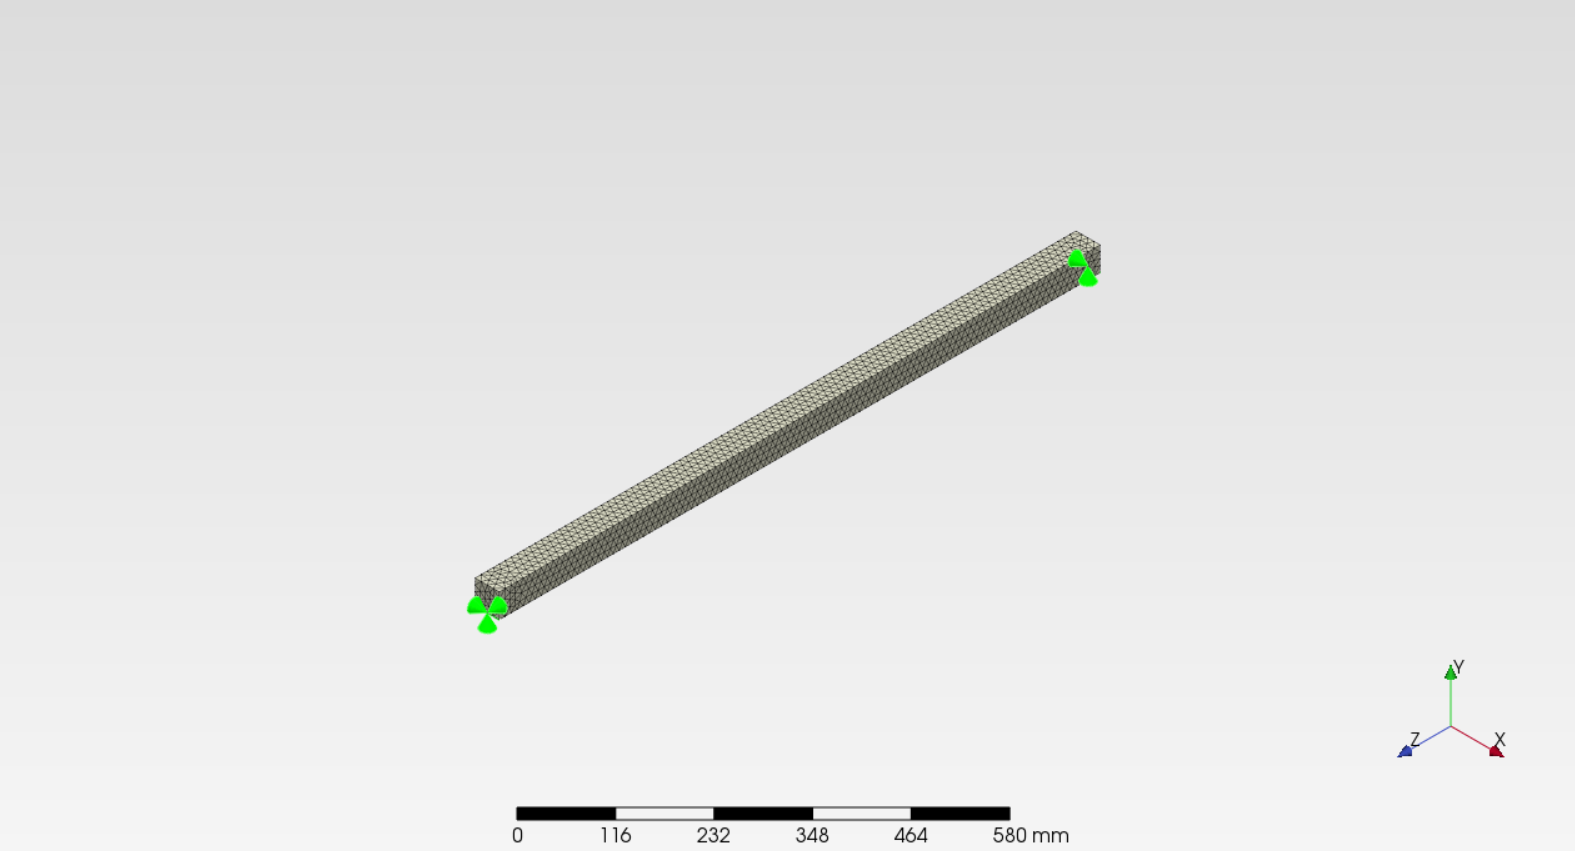
\includegraphics[width=.95\columnwidth]{fig/06-01.png}
	\end{minipage}
	%
	\begin{minipage}{.49\hsize}
		\caption{解析結果}
		\label{06-02}
		\centering
		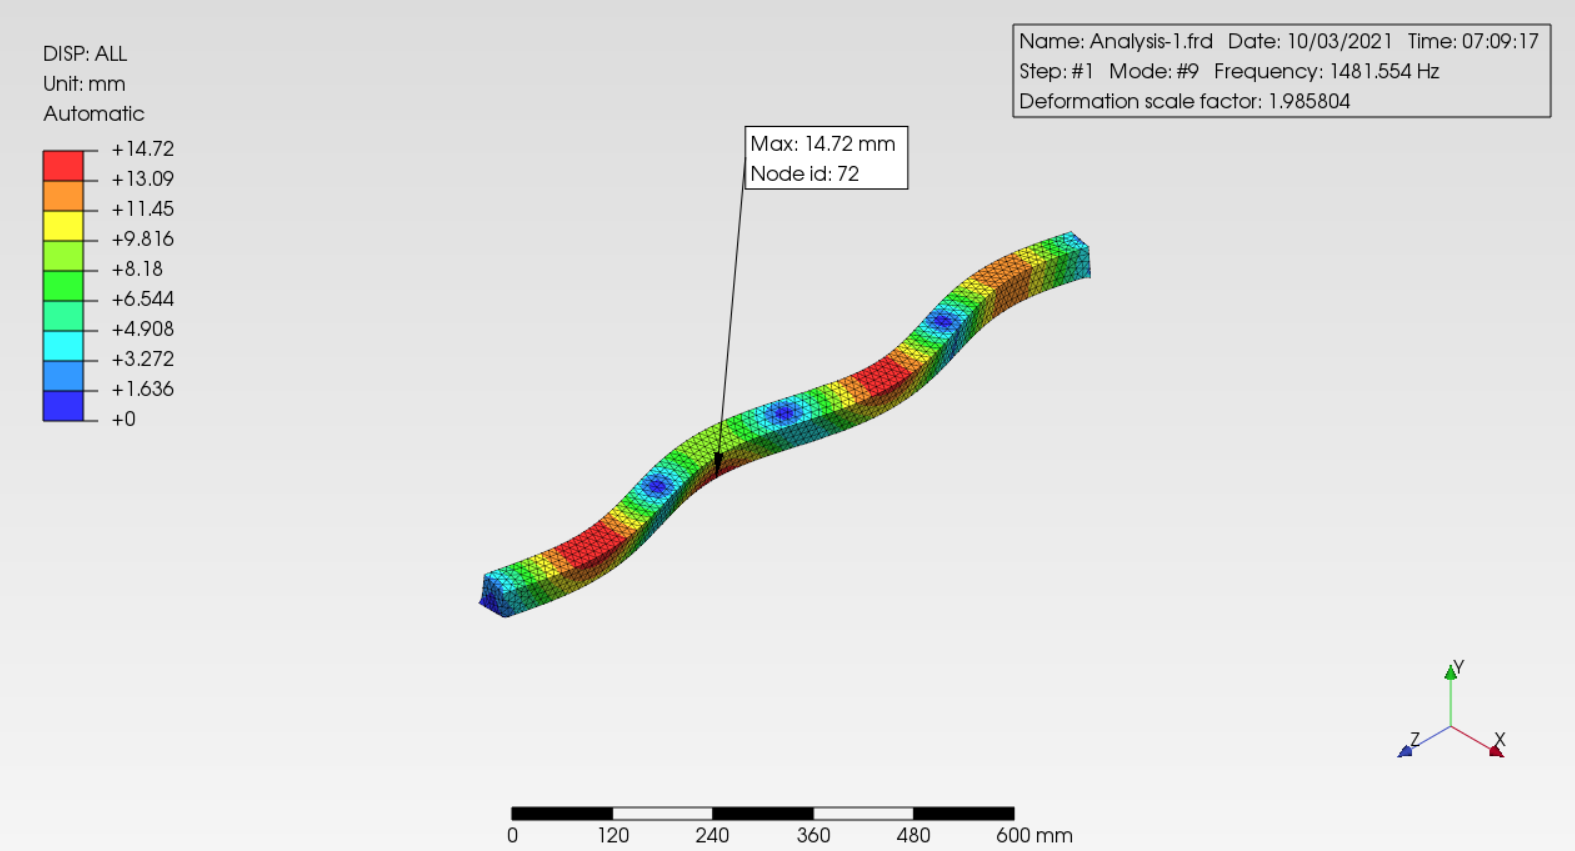
\includegraphics[width=.95\columnwidth]{fig/06-02.png}
	\end{minipage}
\end{figure}
\clearpage
%
\subsection{引張弾塑性プレート}
\begin{figure}[H]
	%
	\begin{minipage}{.59\hsize}
		\begin{itemize}
			\item モデル形状(プレートサイズ:300x150mm、穴の直径:60mm、厚さ:10mmの1/4モデル)
			\item 最大要素サイズ:4mm
			\item 材料定数
			      \begin{itemize}
				      \item ヤング率:210,000MPa
				      \item ポアソン比:0.3
			      \end{itemize}
			\item 境界条件:プレートが引っ張られる側に-200MPaの圧力荷重
		\end{itemize}
	\end{minipage}
	%
	\begin{minipage}{.39\hsize}
		\begin{table}[H]
			\centering
			\caption{塑性定義のデータポイント}
			\begin{tabular}{@{}cc@{}}
				\toprule
				降伏応力 {[}MPa{]} & 塑性ひずみ{[}-{]} \\ \midrule
				235                & 0                 \\
				335                & 0.12              \\ \bottomrule
			\end{tabular}
		\end{table}
	\end{minipage}
\end{figure}
\vspace{-\baselineskip}
\begin{figure}[H]
	%
	\begin{minipage}{.49\hsize}
		\caption{境界条件}
		\label{07-01}
		\centering
		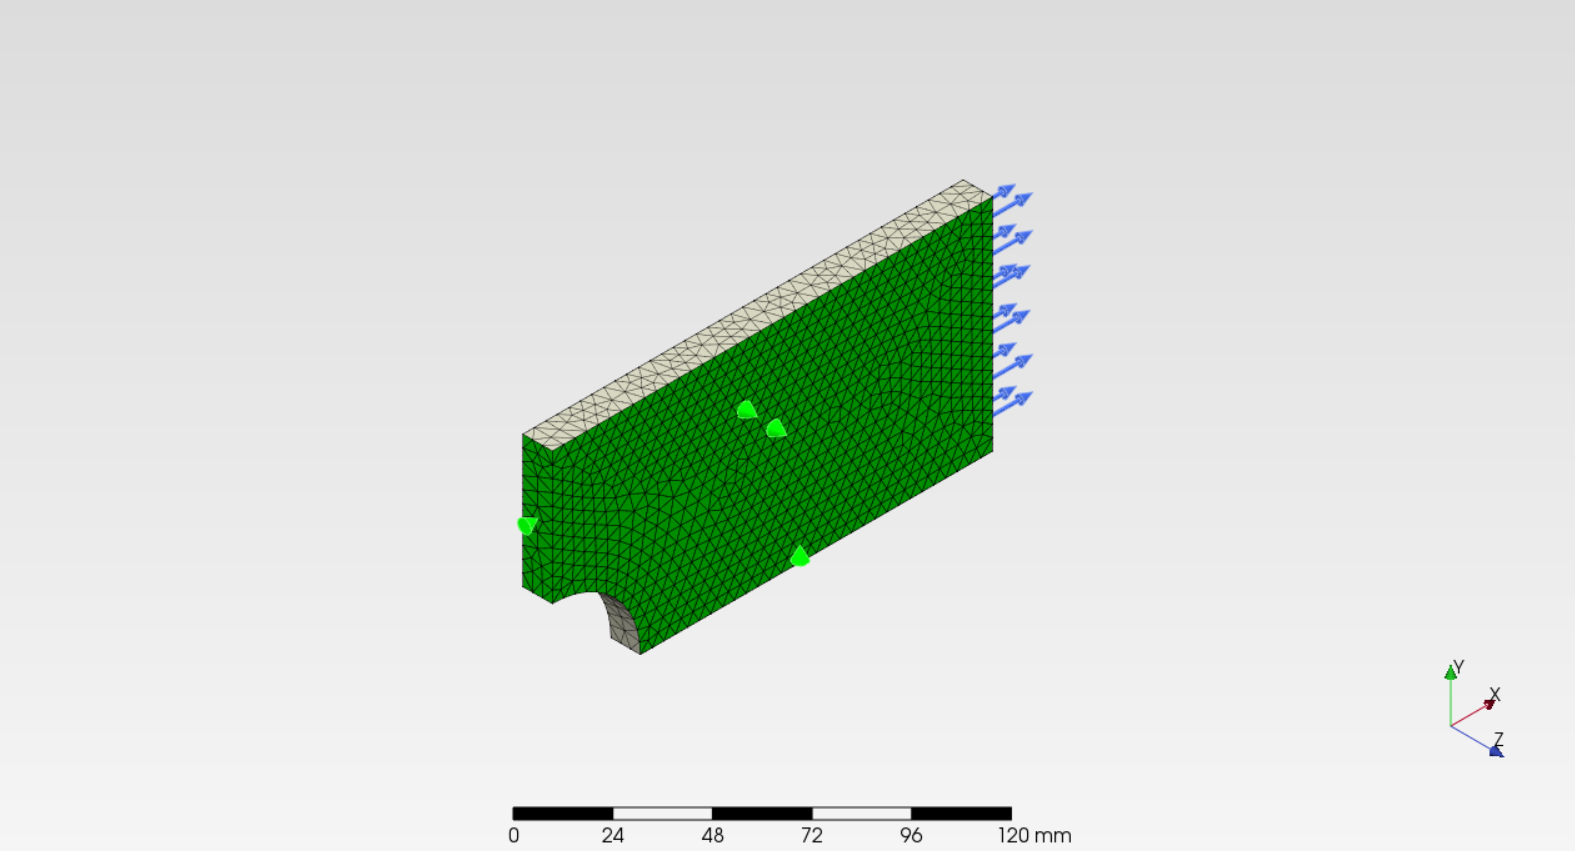
\includegraphics[width=.95\columnwidth]{fig/07-01.png}
	\end{minipage}
	%
	\begin{minipage}{.49\hsize}
		\caption{解析結果}
		\label{07-02}
		\centering
		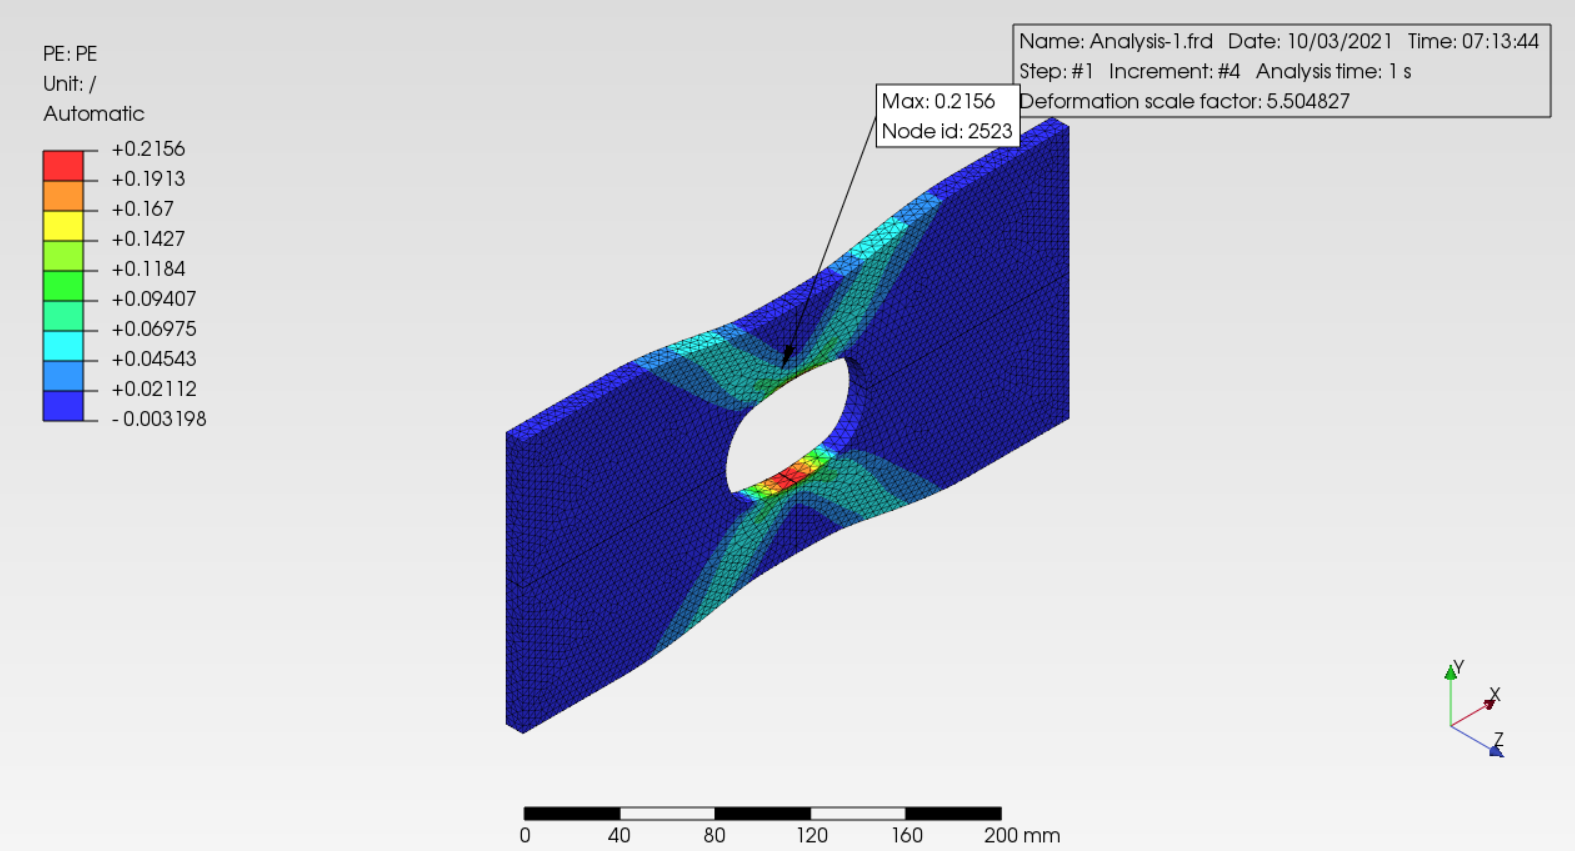
\includegraphics[width=.95\columnwidth]{fig/07-02.png}
	\end{minipage}
\end{figure}
\clearpage
%
\subsection{2つの球のヘルツ接触}
\begin{itemize}
	\item モデル形状(半径50mmの2つの球の1/8モデル)
	\item 最大要素サイズ:5mm(接触領域に0.5mm)
	\item 材料定数
	      \begin{itemize}
		      \item ヤング率:200,000MPa
		      \item ポアソン比:0.3
	      \end{itemize}
	\item 拘束条件:球が互いに押し付けられるように、上面と下面に2mmと-2mmの変位を設定
	\item 大変形:オン
\end{itemize}
\vspace{-\baselineskip}
\begin{figure}[H]
	%
	\begin{minipage}{.49\hsize}
		\caption{境界条件}
		\label{08-01}
		\centering
		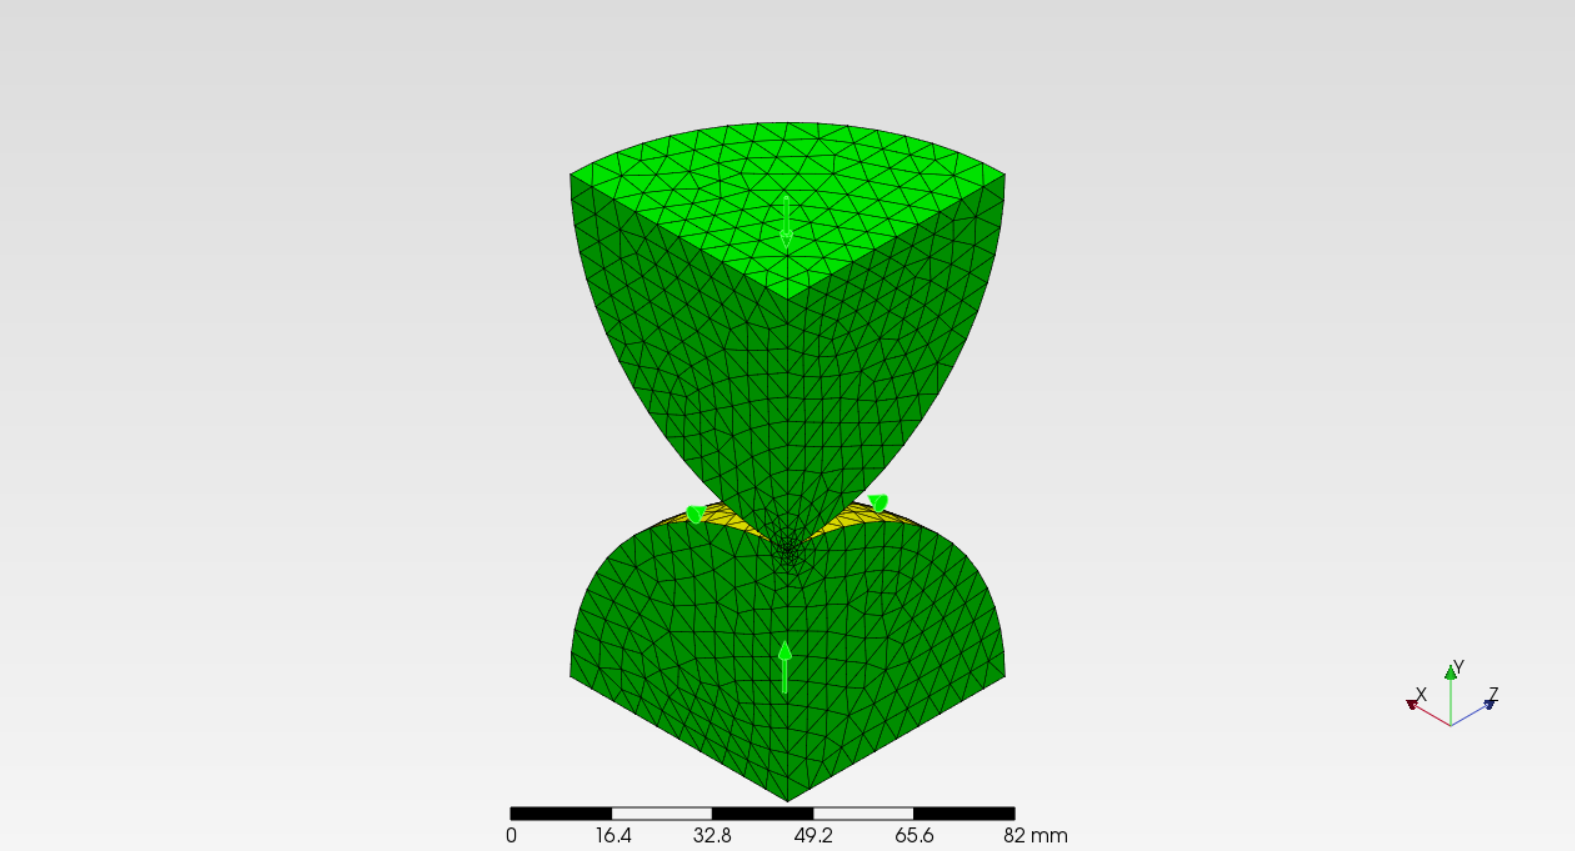
\includegraphics[width=.95\columnwidth]{fig/08-01.png}
	\end{minipage}
	%
	\begin{minipage}{.49\hsize}
		\caption{解析結果}
		\label{08-02}
		\centering
		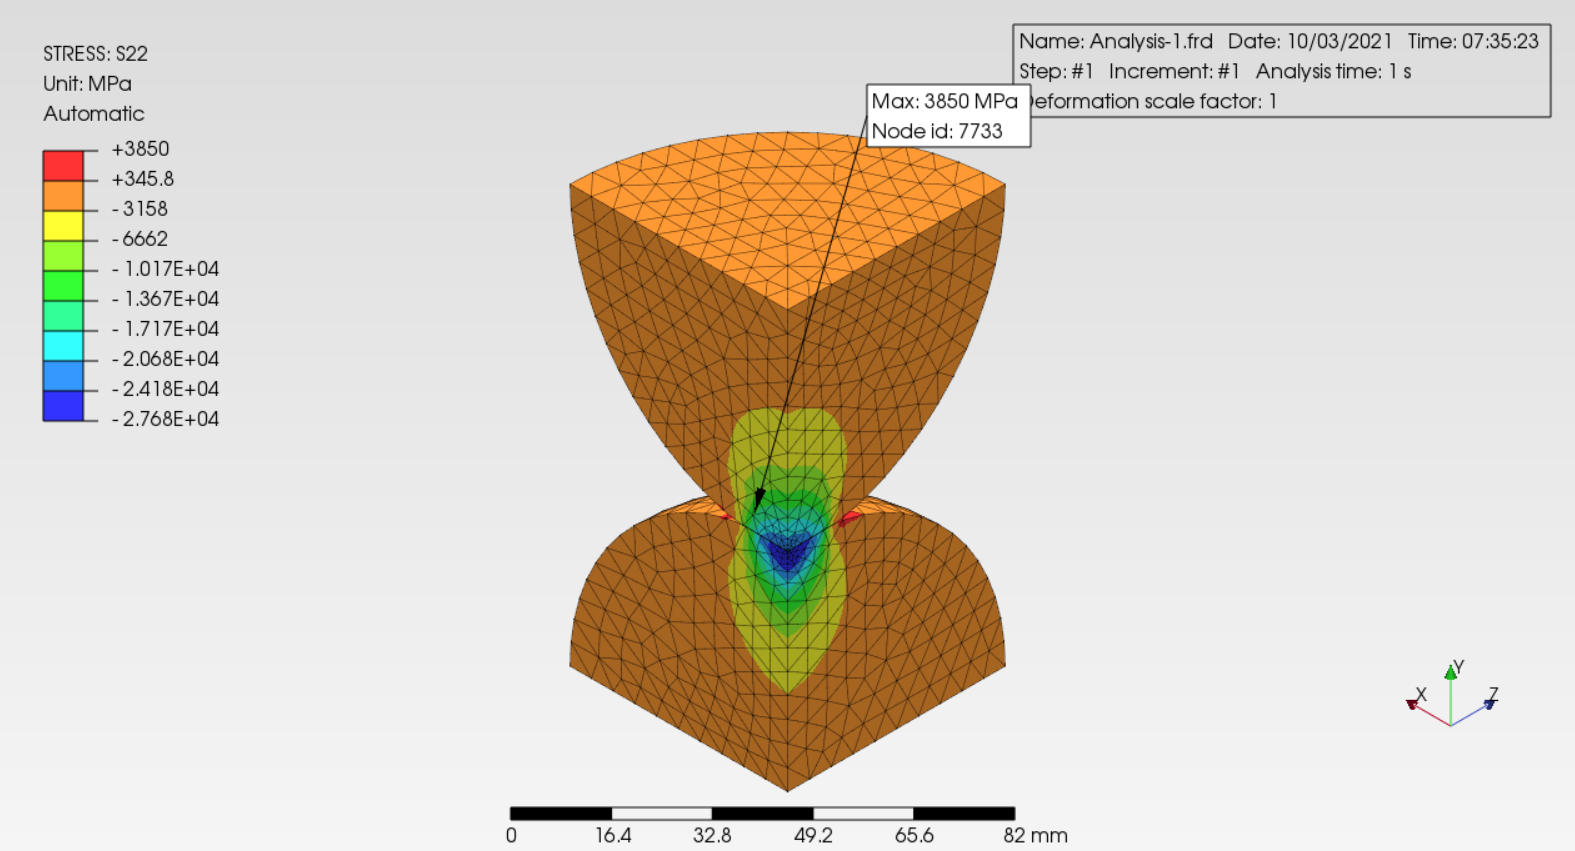
\includegraphics[width=.95\columnwidth]{fig/08-02.png}
	\end{minipage}
\end{figure}
\clearpage
%
\subsection{円筒シェルの座屈}
\begin{itemize}
	\item モデル形状(直径: 300 mm、長さ:600mm、厚さ:5mm)
	\item 最大要素サイズ:10mm(四角形メッシュ)
	\item 材料定数
	      \begin{itemize}
		      \item ヤング率:210,000MPa
		      \item ポアソン比:0.3
	      \end{itemize}
	\item 荷重条件:座標(0, 0, 600)の基準点からシェルの上端と剛体拘束を定義し、基準点に-1N
	\item 拘束条件:シェルの下部エッジを固定
\end{itemize}
\vspace{-\baselineskip}
\begin{figure}[H]
	%
	\begin{minipage}{.49\hsize}
		\caption{境界条件}
		\label{09-01}
		\centering
		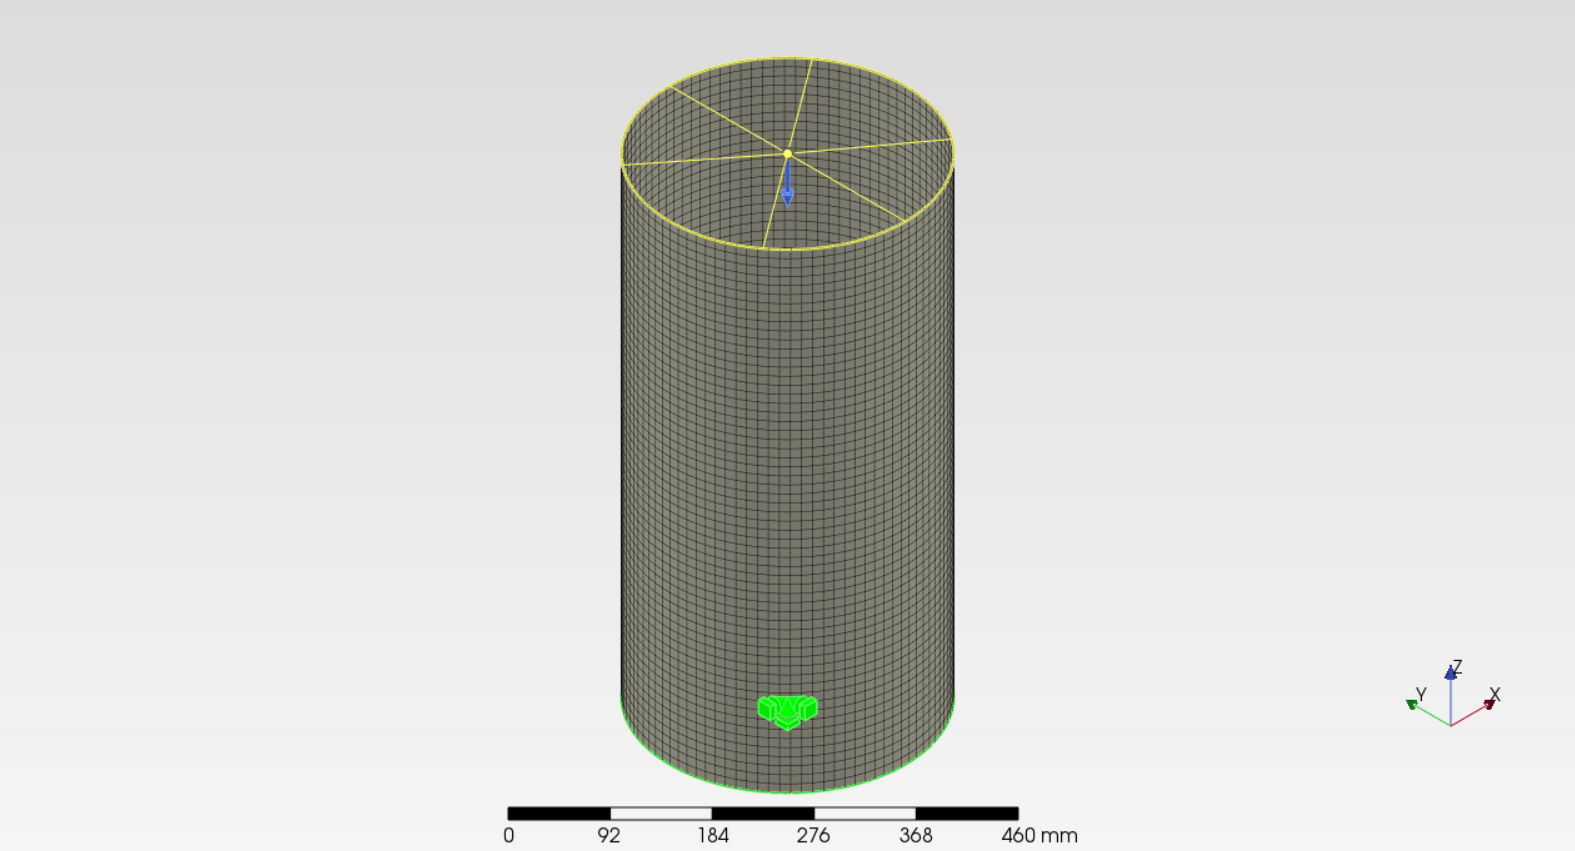
\includegraphics[width=.95\columnwidth]{fig/09-01.png}
	\end{minipage}
	%
	\begin{minipage}{.49\hsize}
		\caption{解析結果}
		\label{09-02}
		\centering
		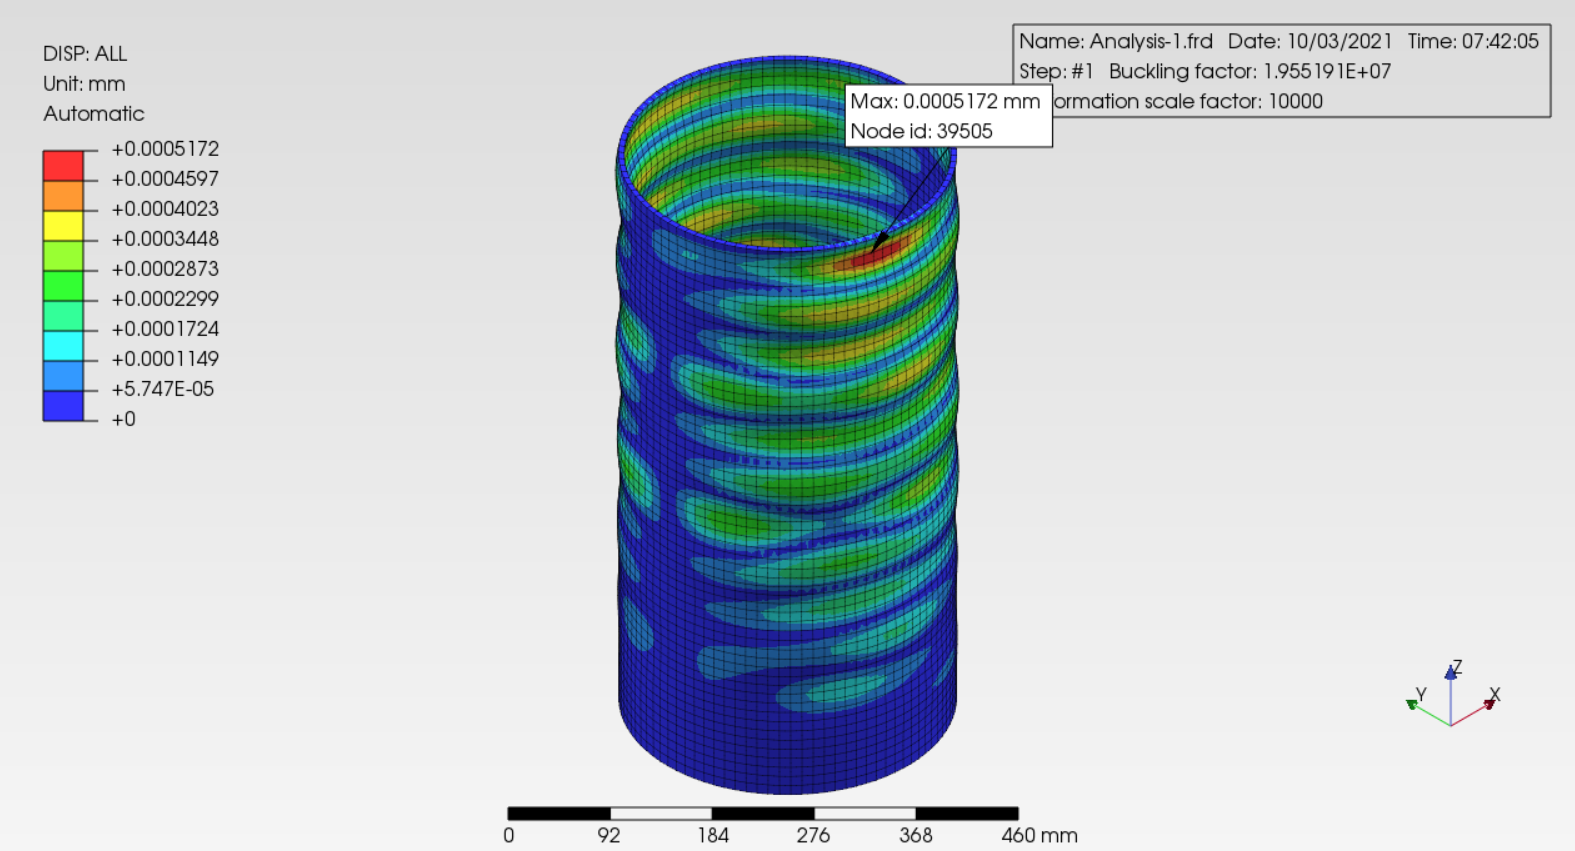
\includegraphics[width=.95\columnwidth]{fig/09-02.png}
	\end{minipage}
\end{figure}
\clearpage
%
\subsection{単純支持されたプレートの圧縮時の座屈}
\begin{itemize}
	\item モデル形状(200x150mm、厚さ:4mm)
	\item 最大要素サイズ:5mm(四角形メッシュ)
	\item 材料定数
	      \begin{itemize}
		      \item ヤング率:200,000MPa
		      \item ポアソン比:0.3
	      \end{itemize}
	\item 拘束条件:プレートのすべてのエッジ(U3を固定)、垂直な2つのエッジに法線方向を拘束
	\item 荷重条件:法線方向を拘束したエッジと反対側のエッジにシェルエッジ荷重を1N/mm
\end{itemize}
\vspace{-\baselineskip}
\begin{figure}[H]
	%
	\begin{minipage}{.49\hsize}
		\caption{境界条件}
		\label{10-01}
		\centering
		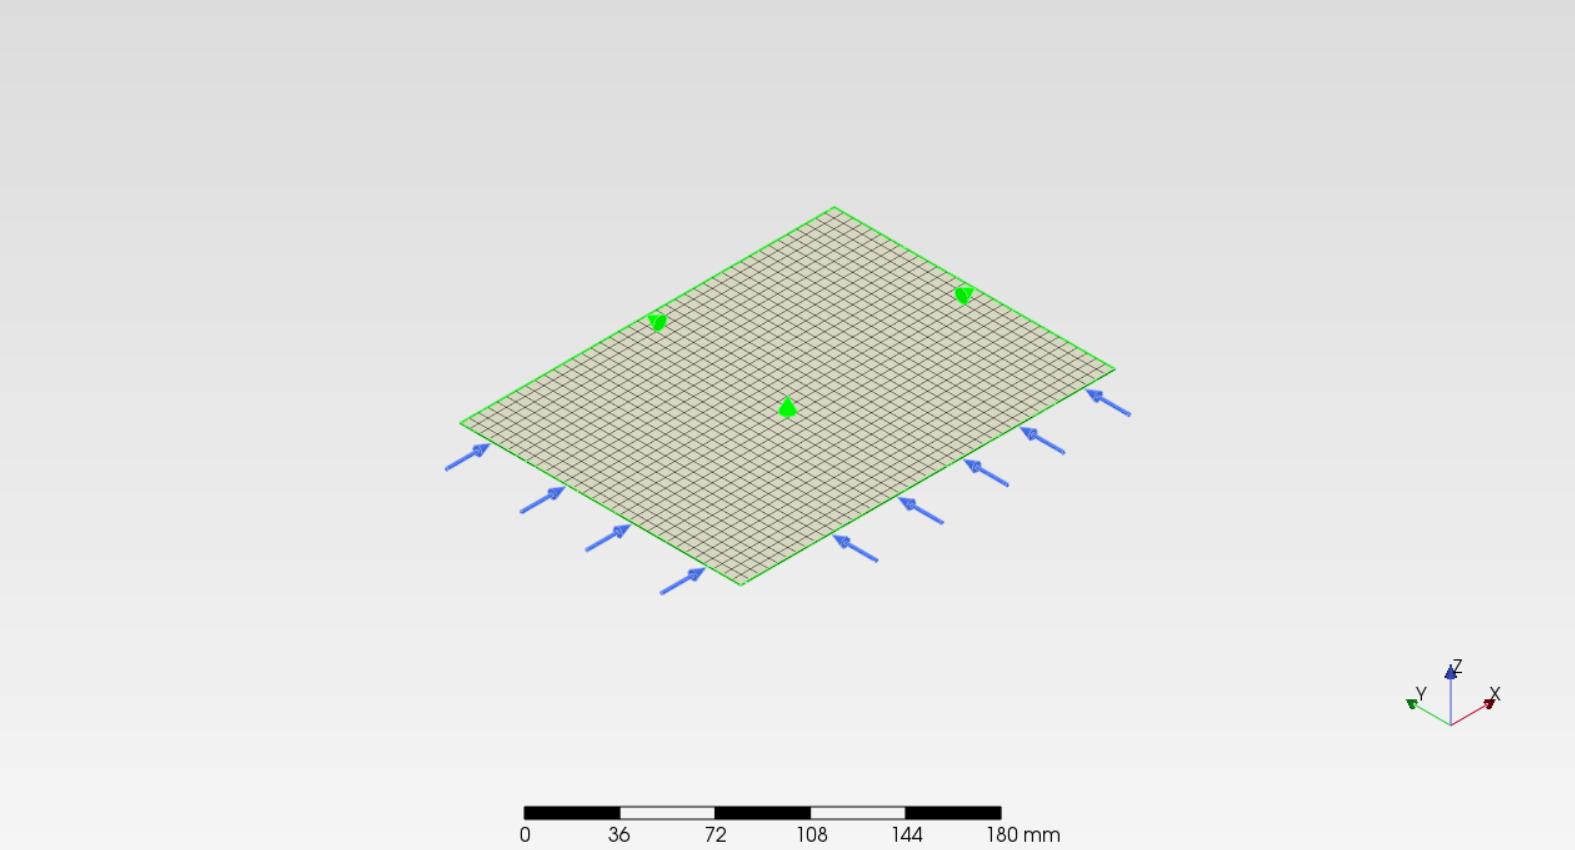
\includegraphics[width=.95\columnwidth]{fig/10-01.png}
	\end{minipage}
	%
	\begin{minipage}{.49\hsize}
		\caption{解析結果}
		\label{10-02}
		\centering
		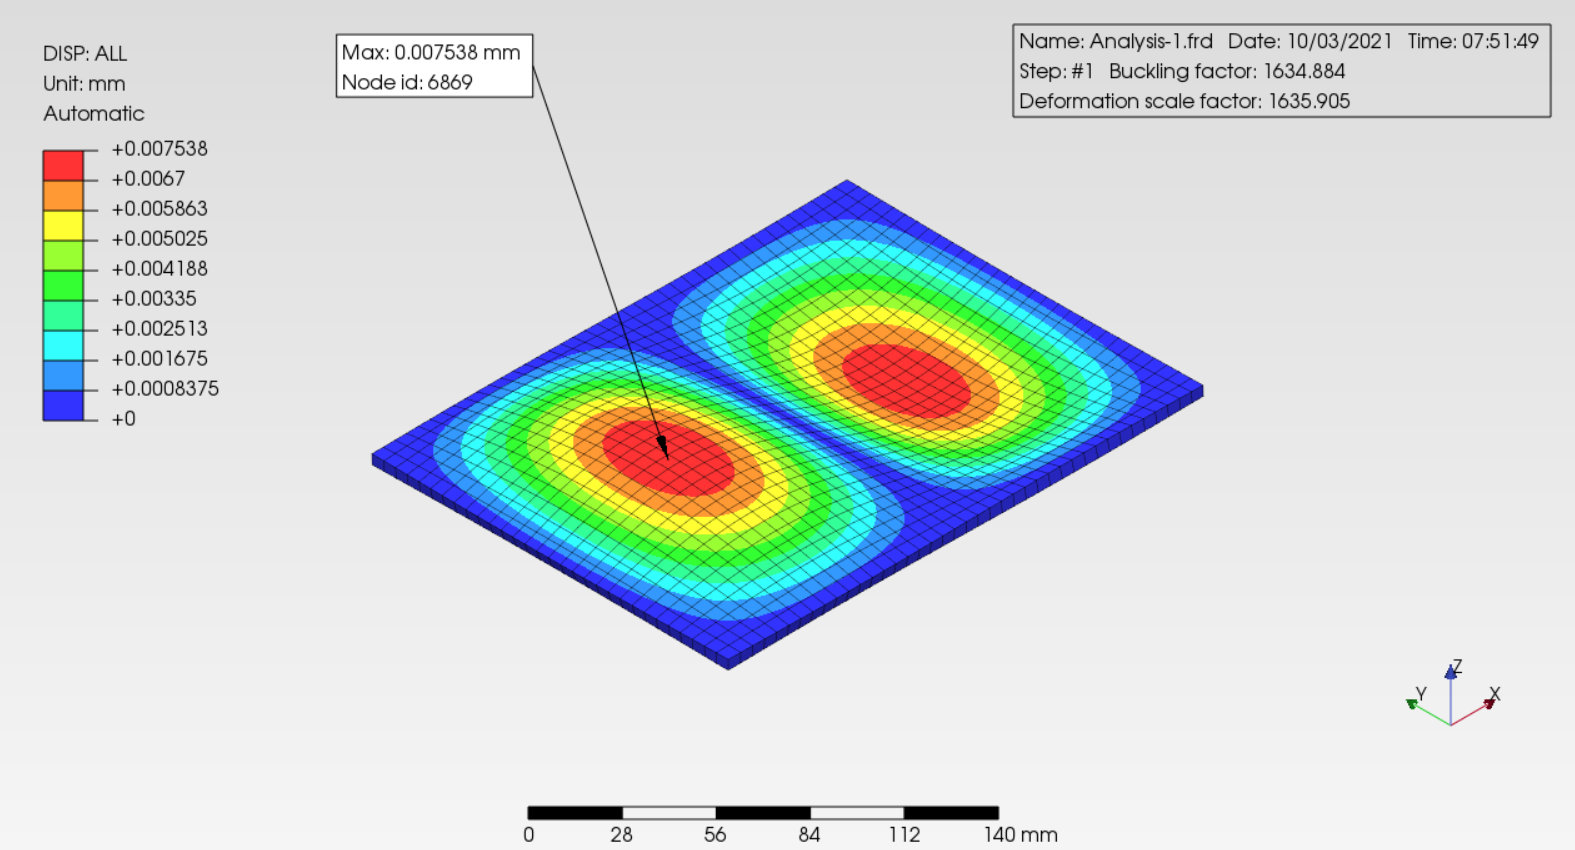
\includegraphics[width=.95\columnwidth]{fig/10-02.png}
	\end{minipage}
\end{figure}
\clearpage
%
\subsection{断熱パイプラインの熱伝達}
\begin{itemize}
	\item モデル形状(外径:57mm、内径: 50mm、断熱材の厚さ: 28mm、長さ: 200mm)
	\item 最大要素サイズ:断熱材は2mm、パイプは3mm
	\item 材料定数
	      \begin{itemize}
		      \item パイプ:熱伝導率45mW/(mm-°C)
		      \item 断熱材:0.05mW/(mm-°C)
	      \end{itemize}
	\item 温度条件
	      \begin{itemize}
		      \item 断熱材の外:表面温度20℃、熱伝達率を0.015 mW/(mm2-°C)
		      \item パイプの内側:表面温度-30℃、熱伝達率は0.8mW/(mm2-°C)
	      \end{itemize}
\end{itemize}
\vspace{-\baselineskip}
\begin{figure}[H]
	%
	\begin{minipage}{.49\hsize}
		\caption{境界条件}
		\label{11-01}
		\centering
		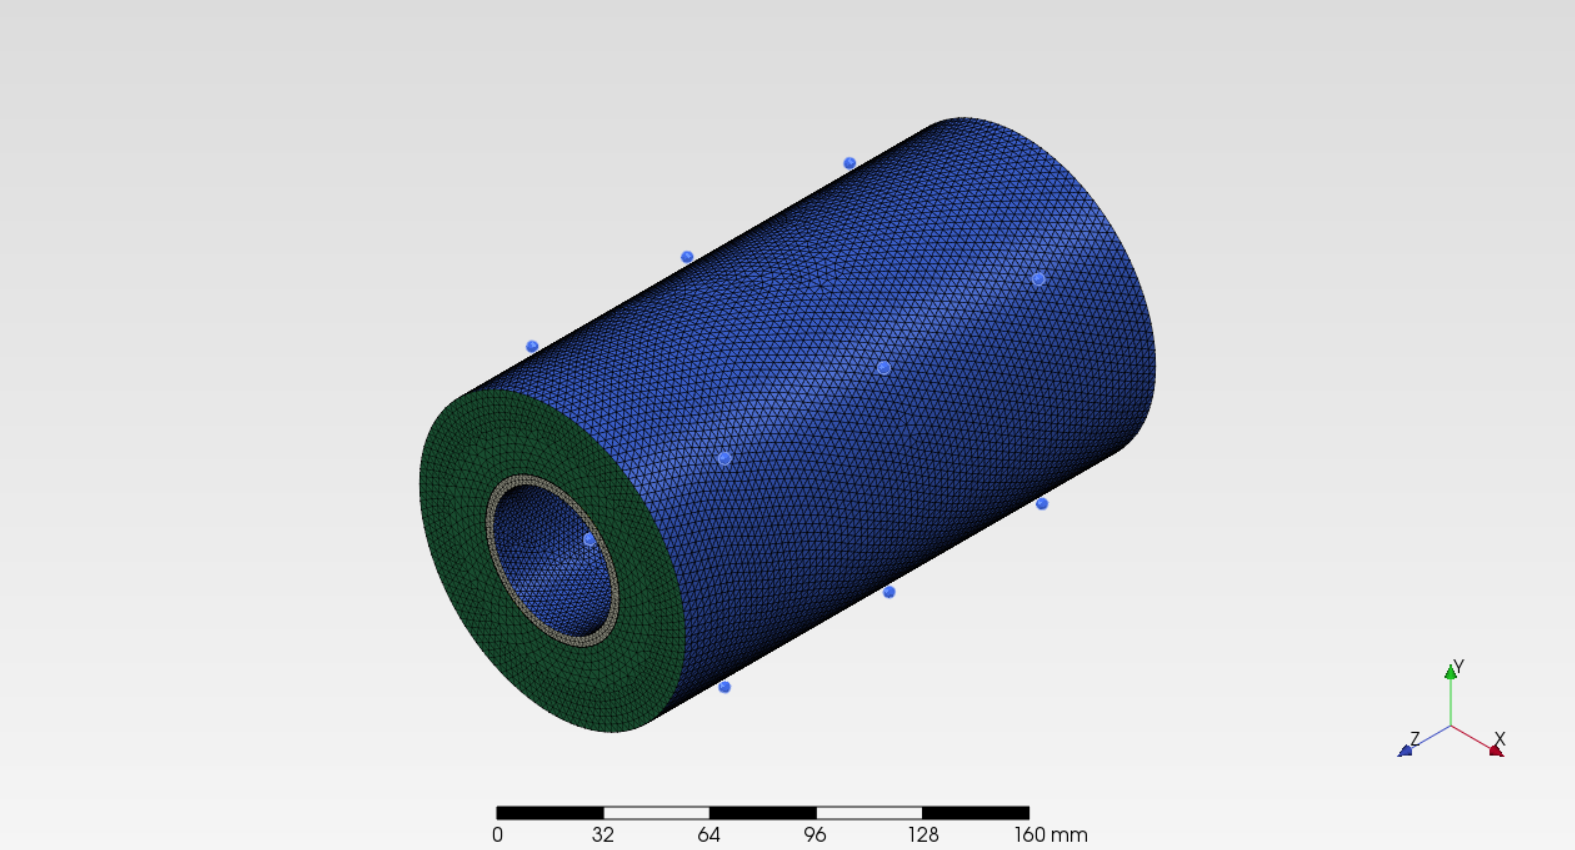
\includegraphics[width=.95\columnwidth]{fig/11-01.png}
	\end{minipage}
	%
	\begin{minipage}{.49\hsize}
		\caption{解析結果}
		\label{11-02}
		\centering
		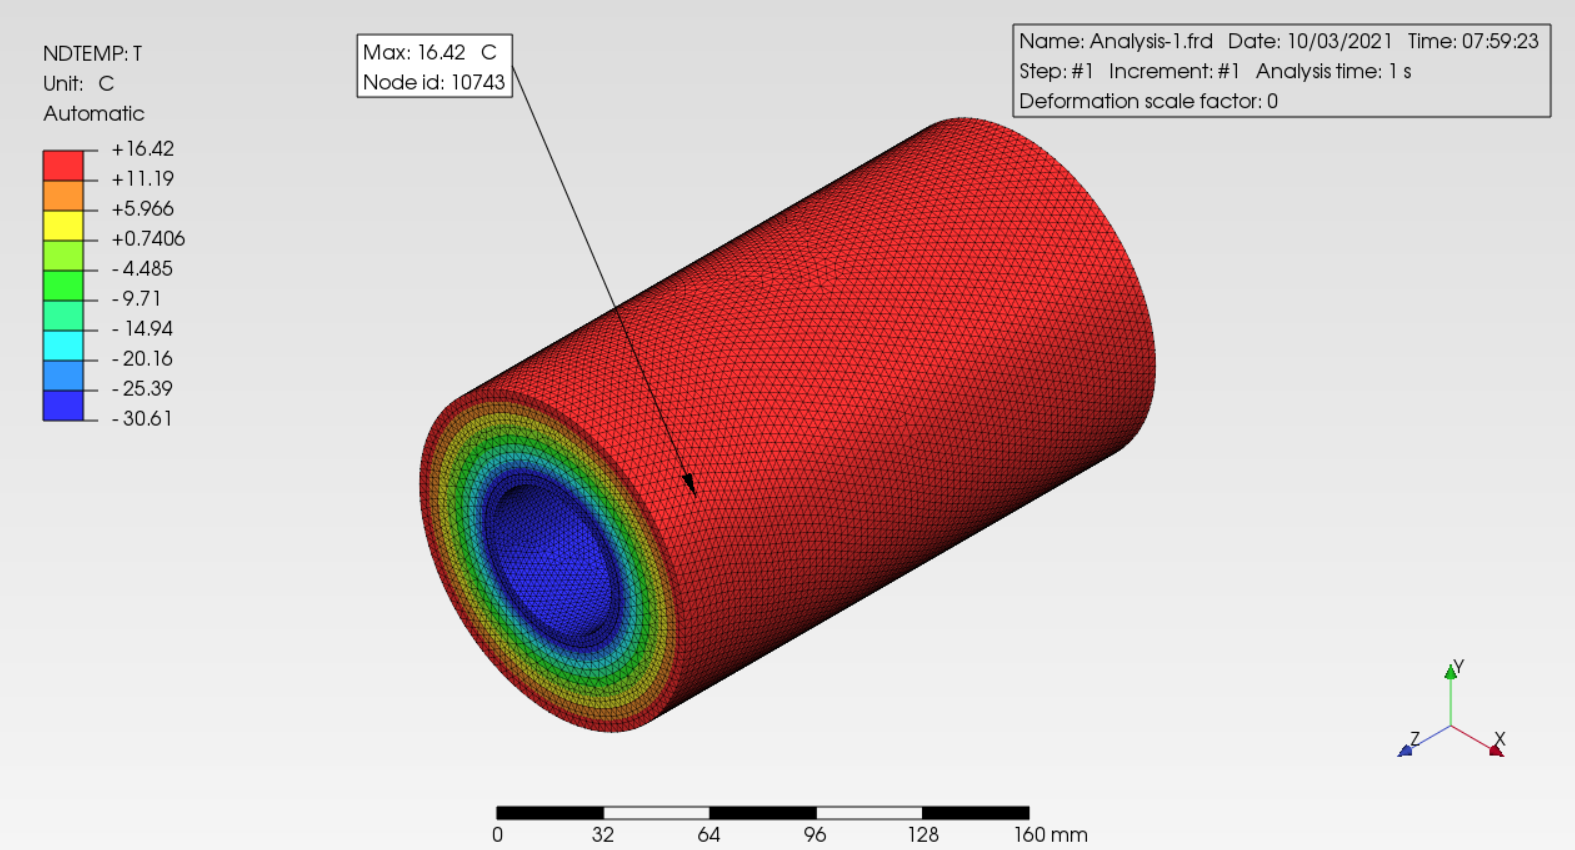
\includegraphics[width=.95\columnwidth]{fig/11-02.png}
	\end{minipage}
\end{figure}
\clearpage
%
\subsection{バイメタル小片の熱構造解析}
\begin{itemize}
	\item モデル形状(2本の梁(120x20x4mm)を互いに重ねて配置したもの)
	\item 最大要素サイズ:1mm
	\item 材料定数
	      \vspace{-.5\baselineskip}
	      \begin{table}[H]
		      \centering
		      \begin{tabular}{@{}lrrrrr@{}}
			      \toprule
			      材料   & ヤング率{[}MPa{]} & ポアソン比 & 熱伝導率 & 熱膨張率 & 零温度{[}℃{]} \\ \midrule
			      Copper & 130,000           & 0.34       & 385      & 17e-6.0  & 20            \\
			      Steel  & 210,000           & 0.3        & 45       & 12.3e-6  & 20            \\ \bottomrule
		      \end{tabular}
	      \end{table}
	      \vspace{-\baselineskip}
	\item 固定条件:両方の梁の背面を固定
	\item 温度条件:80℃
\end{itemize}
\vspace{-\baselineskip}
\begin{figure}[H]
	%
	\begin{minipage}{.49\hsize}
		\caption{境界条件}
		\label{12-01}
		\centering
		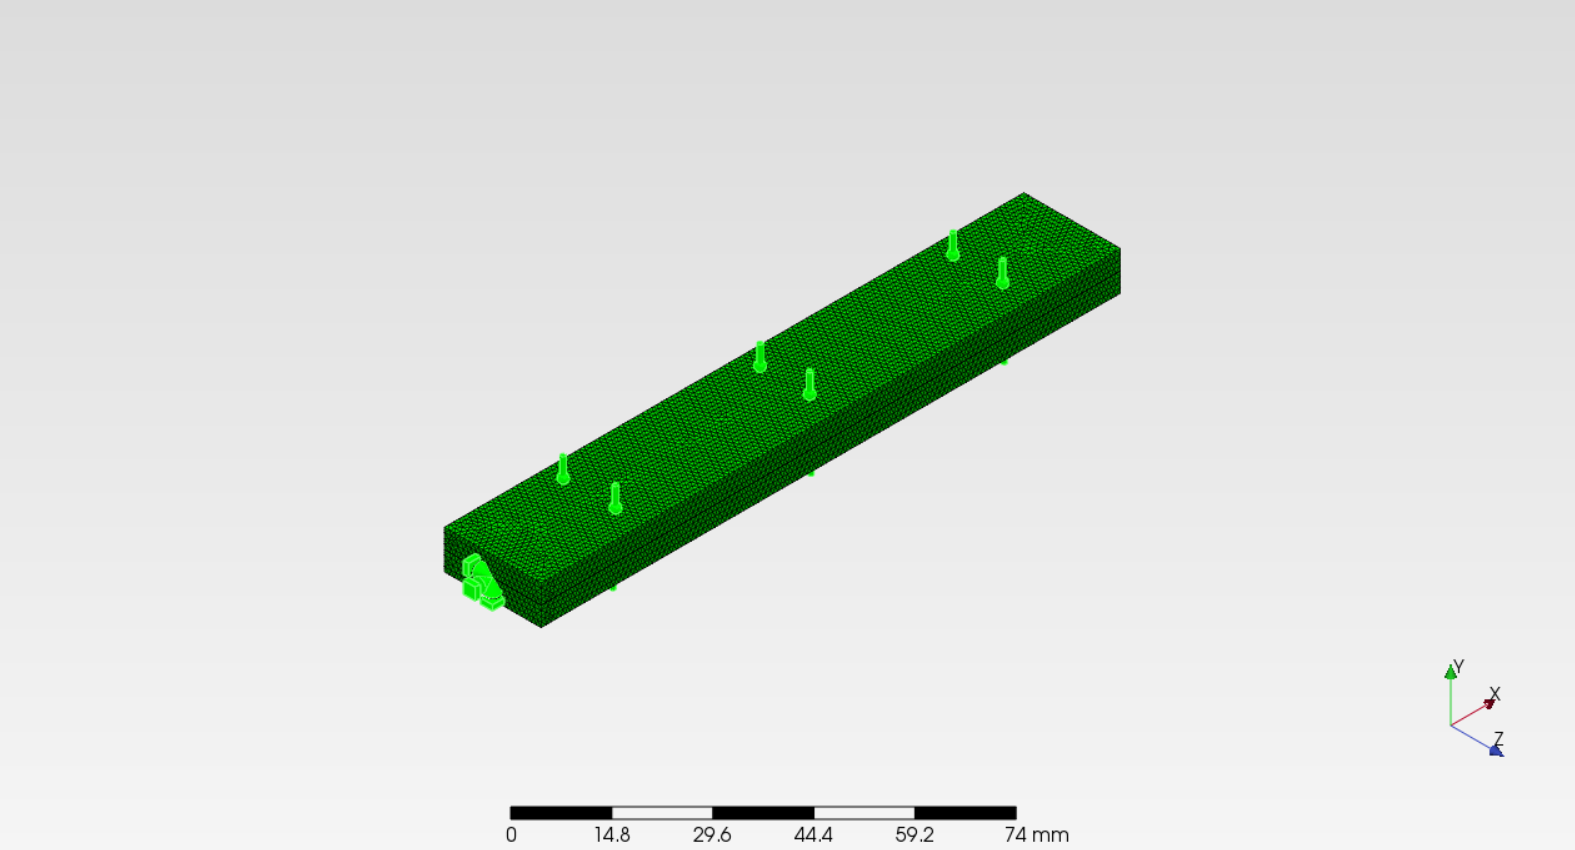
\includegraphics[width=.95\columnwidth]{fig/12-01.png}
	\end{minipage}
	%
	\begin{minipage}{.49\hsize}
		\caption{解析結果}
		\label{12-02}
		\centering
		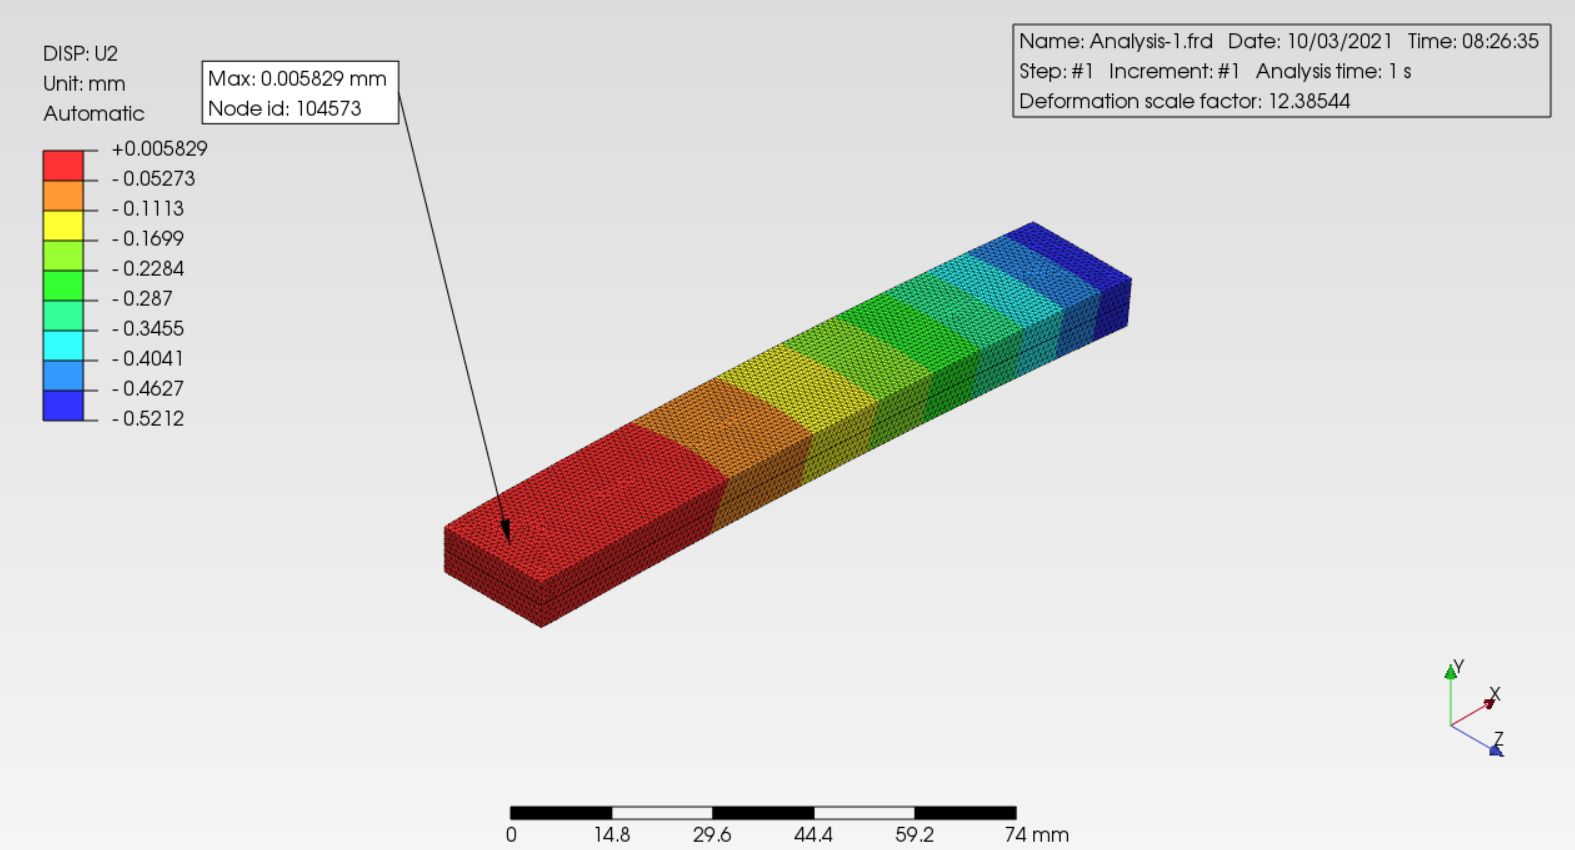
\includegraphics[width=.95\columnwidth]{fig/12-02.png}
	\end{minipage}
\end{figure}
\clearpage
%
\section{solverとCPU数の比較}
\ref{sec:6.3}の楕円形の棒のねじりを各solverとCPU数で計算速度を比較しました。
\begin{table}[H]
\centering
\begin{tabular}{@{}rrrrrrr@{}}
\toprule
CPU数 & Default & PaStix & Pardiso & SPOOLES & Iterative Scaling & Iterative Choleski \\ \midrule
1      & 64.47   & 62.70  & 63.27   & 64.26   & 62.73             & 64.34              \\
2      & 53.14   & 48.03  & 48.93   & 49.08   & 49.39             & 48.80              \\
3      & 44.92   & 41.50  & 41.99   & 40.98   & 41.27             & 41.10              \\
4      & 35.22   & 35.36  & 35.48   & 35.09   & 35.30             & 35.33              \\
5      & 32.86   & 32.81  & 32.74   & 32.47   & 32.84             & 33.42              \\
6      & 31.87   & 32.01  & 30.76   & 31.43   & 31.34             & 32.15              \\ \bottomrule
\end{tabular}
\end{table}
\begin{thebibliography}{9}
	\bibitem Wikipedia,Calculix,\href{https://en.wikipedia.org/wiki/Calculix}{https://en.wikipedia.org/wiki/Calculix},(Accessed on 10/03/2021)
	\bibitem Matej Borovinšek,PrePoMax,\href{https://prepomax.fs.um.si/}{https://prepomax.fs.um.si/},(Accessed on 10/03/2021)
	\bibitem Jakub Michalski・Matej Borovinšek,PrePoMax v1.1.0 Examples,\href{https://prepomax.fs.um.si/wp-content/uploads/2021/09/2021.09.07-PrePoMax-v1.1.0-examples-manual.pdf}{https://prepomax.fs.um.si/wp-content/uploads/2021/09/2021.09.07-PrePoMax-v1.1.0-examples-manual.pdf}
	\bibitem Ihor Rokach,Instrukcje, HowTo PrePoMax
	\bibitem XSim,CalculiX 使い方メモ,\href{https://www.xsim.info/articles/CalculiX/How-to-use-CalculiX.html}{https://www.xsim.info/articles/CalculiX/How-to-use-CalculiX.html},(Accessed on 10/03/2021)
	\bibitem 柴田 良一,「PrePoMax」ではじめる実線構造解析,工学社(2018).
\end{thebibliography}
\end{document}